% Volume III chapter: Chebyshev's error, Levy measures and the Thorin ladder. Sources: misc/reviews/nick-chebyshev-thorin/chebyshev_thorin_for_vadim/book_chapter/chebyshev_thorin_volume3.tex lines 1 to 882 (rung one, the upper and lower ladders, thm:finite and the code section reduced to one section or cut); referee reports CT1 (M1 to M9) and CT2 (M1 to M9); verification misc/vol3/verify/CT/results.md. 17 Nov 2026. Extended 17 Nov 2026 with the five new sections of the revised note (misc/reviews/nick-chebyshev-thorin-v2, lines 849 to 1325; referee CT3, verification CT3) and the new parts of the chapter misc/reviews/nick-cheb1850-gamma/cheb1850/chebyshev_identity_chapter.tex (referee C1850, verification C1850). New bibliography entry in ch/nc_v3_cheb_bib.tex (Littlewood12). Figures added to fig/v3: fig_budget, fig_yamazato_split, fig_symmetric_kernel, fig_mobius_rate. Coordinator: ct:thm:budget is also the ledger identity of the Vol III ledger chapter (misc/vol3/ledger/SYNTHESIS.md item 1); ch/nc_v3_final.tex:89 still says nonnegative running sums may be necessary and should cite ct:thm:hier.
% Coordinator notes: label prefix ct:; no new bibliography file (Montgomery 1980, Rubinstein and Sarnak, Sylvester, Malmsten, Wintner 1935 and Diamond and Erdos are named in the text without a key because ch/bib.tex and misc/vol3/bib_new.tex have no entry; add keys if wanted). Figures copied to fig/v3: fig_weights, ch_bondesson, ch_uweighted, ch_yamazato, ch_ladder, ch_periodogram, ch_wintner, fig_p3_deconv, fig_p4_tail. ch_bondesson is plotted against the note's z = r^2/2 (the caption says so) and should be redrawn in z = r^2. ch_ladder dots, ch_periodogram, ch_wintner, fig_p3_deconv and fig_p4_tail were not recomputed by the verification (% UNVERIFIED). Dropped with the rung one and ladder sections: fig_range3, fig_rung_one, tab:upper, thm:finite, Problem 6, the code section.
\label{ct:ch:cheb}

This chapter reads Chebyshev's two memoirs and the statistics of $\psi(x)-x$ in the language of Thorin measures. Results are from an unrefereed note of Polson (November 2026) unless a source is named. We use the book's chart: the Laplace variable is $u=w^2$, the Thorin variable is $z=r^2$, and the atoms at the centre are $\gamma^2$. The note works in the chart $u=w^2/2$, so every rate below is twice the note's. The symbol $\xi$ is Riemann's, with the factor $\frac12s(s-1)$, and the term $1/s$ of $\xi'/\xi$ sits in the archimedean block, as in equation~\eqref{eq:split}. We write $v_\alpha(r)=\Re\frac{\xi'}{\xi}(\alpha+ir)$ and $b_\alpha=\frac{\xi'}{\xi}(\alpha)$, and $t_\alpha(z)$ for the Thorin density in $z$ (the symbol $T_\alpha$ is the random variable of Volume I). Status words follow the book: proved, computed (floating point), certified (ball arithmetic), conditional, heuristic, open. The half plane $\frac78$ of \cite{OAI26a} is used once, in Section~\ref{ct:sec:budget}.

What the chapter contains, and what it does not.
\begin{enumerate}
\item The compensated L\'evy measure of $\log\xi$ is Chebyshev's error measure corrected for the trivial zeros (Proposition~\ref{ct:prop:levy}, proved and checked numerically), and for $\alpha>1$ the Thorin density at level $\alpha$ is its tapered transform (Theorem~\ref{ct:thm:dictionary}).
\item Chebyshev's 1850 Gamma ratio gives a generalised gamma convolution with an explicit Thorin density and tail constant $A=0.92129$ (Theorem~\ref{ct:thm:chebggc}, proved). The same computation gives an explicit Thorin density for Bondesson's function $e^{-\gamma\sqrt u}/\Gamma(1+\sqrt u)$ (Corollary~\ref{ct:cor:bondesson}).
\item Yamazato's integer part split applied to Chebyshev's ratio and to the reciprocal Xi function (Theorem~\ref{ct:thm:chebME}, Proposition~\ref{ct:prop:yamxi}), with the limit of the integer crossings as a conjecture (Conjecture~\ref{ct:conj:canonical}).
\item Cram\'er's variance in Thorin form, the periodogram of the normalised error, and the rotor model of its limiting law and tail (computed or heuristic, as marked).
\item A sufficient condition for a signed product of Gamma functions to be a GGC (Theorem~\ref{ct:thm:runningsums}, proved) and a deconvolution that recovers the zeros below $180$ from the primes (computed).
\item The budget form of the Thorin density and the oscillation of Chebyshev's error, the direct form, Yamazato's split at level one and its Bernoulli limit (Sections~\ref{ct:sec:budget} to~\ref{ct:sec:yamcheb}), Chebyshev's identity in the critical strip with a positive even kernel for $\Xi$ (Section~\ref{ct:sec:strip}, Theorem~\ref{ct:thm:symkernel}) and Ramanujan's continuation (Section~\ref{ct:sec:ramanujan}).
\item A strict hierarchy of positivity conditions for signed Gamma products, linear programs on the divisors of $30030$, the law of Chebyshev's variable and the M\"obius limit with its rate criterion (Sections~\ref{ct:sec:hier} to~\ref{ct:sec:mobius}).
\item Rung one and the ladder above it are in Volume I, and under RH below it in Lagarias (1999) \cite{Lagarias} and Garunk\v{s}tis (2002) \cite{Garunkstis02}. Section~\ref{ct:sec:rung} records only what we add.
\end{enumerate}

\section{Chebyshev's two memoirs}\label{ct:sec:memoirs}

Write $\Lambda$ for the von Mangoldt function, $\psi(x)=\sum_{n\le x}\Lambda(n)$, $\theta(x)=\sum_{p\le x}\log p$, and $E(u)=\psi(e^{u})-e^{u}$ for the error on the log scale. The digamma function is written $\psi_\Gamma$.

\subsection{1848: the Abelian theorem at level one}
Chebyshev worked with $\zeta(s)$ for real $s\downarrow1$ only. He proved that if $\pi(x)\log x/x$ has a limit, the limit is $1$. In statistical language this is an Abelian theorem: the Laplace transform
\[
\int_0^\infty e^{-\alpha u}\dd\psi(e^{u})=-\frac{\zeta'}{\zeta}(\alpha)=\frac{1}{\alpha-1}+O(1)
\]
as $\alpha\downarrow1$ fixes the mean of the L\'evy measure at level one, and any pointwise limit must agree with the mean. What Chebyshev lacked was the Tauberian step, which needs the absence of zeros on $\Re s=1$.

\subsection{1850: the Gamma ratio}
Let $T(x)=\sum_{n\le x}\log n=\log\lfloor x\rfloor!$. Grouping the prime factors of $n!$ gives $T(x)=\sum_{n\le x}\psi(x/n)$. Put $c=(1,\tfrac12,\tfrac13,\tfrac15,\tfrac1{30})$, $\varepsilon=(1,-1,-1,-1,1)$ and
\[
U(t)=\sum_{k}\varepsilon_k\lfloor c_k t\rfloor
=\lfloor t\rfloor-\lfloor t/2\rfloor-\lfloor t/3\rfloor-\lfloor t/5\rfloor+\lfloor t/30\rfloor,\qquad
u(n)=U(n)-U(n-1).
\]
Then
\begin{equation}\label{ct:eq:cheb}
\sum_{n\le x}u(n)\,\psi\!\left(\frac{x}{n}\right)=\sum_k\varepsilon_k T(c_kx)
=\log\frac{\lfloor x\rfloor!\,\lfloor x/30\rfloor!}{\lfloor x/2\rfloor!\,\lfloor x/3\rfloor!\,\lfloor x/5\rfloor!}.
\end{equation}

\begin{proposition}[Chebyshev 1850]\label{ct:prop:cheb1850}
(i) $u(n)=1-[2\mid n]-[3\mid n]-[5\mid n]+[30\mid n]$, $u$ has period $30$, and $U(t)\in\{0,1\}$ for all $t\ge0$.
(ii) $\sum_k\varepsilon_kc_k=0$ and $A:=\sum_k\varepsilon_kc_k\log c_k=\log\dfrac{2^{1/2}3^{1/3}5^{1/5}}{30^{1/30}}=0.921292\ldots$
(iii) The right side of \eqref{ct:eq:cheb} is $Ax+O(\log x)$, hence $\psi(x)-\psi(x/6)\le Ax+O(\log x)\le\psi(x)$ and
\[
A\le\liminf\frac{\psi(x)}{x}\le\limsup\frac{\psi(x)}{x}\le\frac65A=1.10555\ldots
\]
\end{proposition}

\begin{proof}
(i) is a check over one period (and was checked numerically for $t<3000$). (ii) is arithmetic. For (iii), Stirling gives $\sum_k\varepsilon_kT(c_kx)=x\sum_k\varepsilon_kc_k\log(c_kx)-x\sum_k\varepsilon_kc_k+O(\log x)=Ax+O(\log x)$ by (ii). Since $U\in\{0,1\}$ with $U(t)=1$ for $1\le t<6$, Abel summation gives $\psi(x)-\psi(x/6)\le\sum u(n)\psi(x/n)\le\psi(x)$. Iterating the left inequality over $x,x/6,x/36,\ldots$ gives the upper bound.
\end{proof}

\begin{figure}[t]
\centering
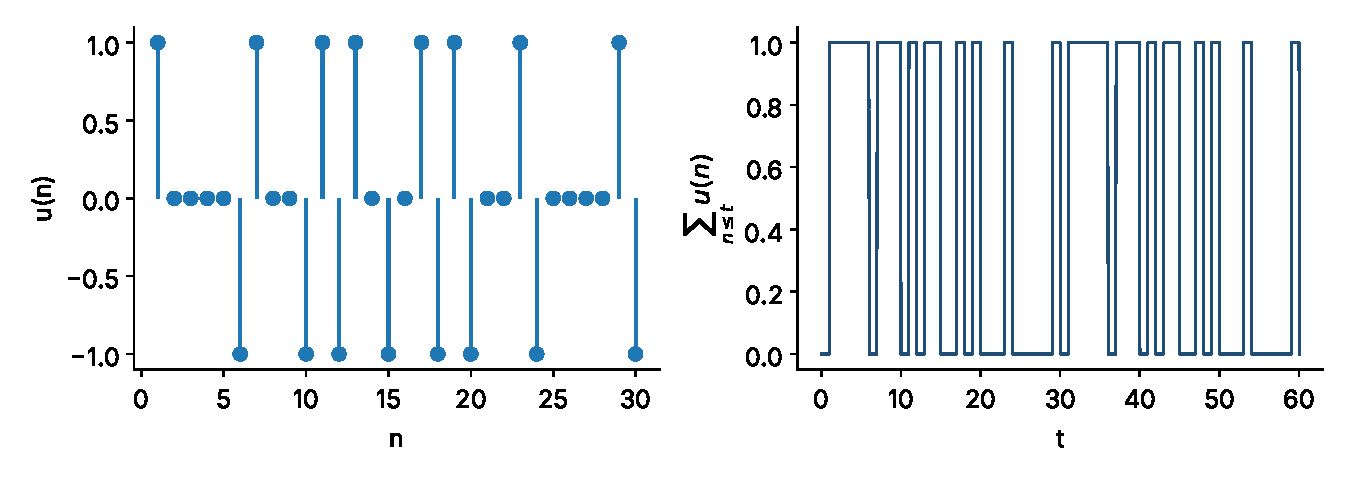
\includegraphics[width=\textwidth]{fig/v3/fig_weights.pdf}
\caption{Chebyshev's weights $u(n)$ over one period (left) and the floor combination $U(t)$, which takes only the values $0$ and $1$ (right).}
\label{ct:fig:weights}
\end{figure}

Two facts will matter below. The condition $\sum\varepsilon_kc_k=0$ is the condition $P(1)=0$ for the Dirichlet polynomial $P(s)=\sum_k\varepsilon_kc_k^{s}=1-2^{-s}-3^{-s}-5^{-s}+30^{-s}$, which satisfies $\sum_nu(n)n^{-s}=\zeta(s)P(s)$ and so cancels the pole of $\zeta$. The condition $U\in\{0,1\}$ is a positivity condition. In Section~\ref{ct:sec:gamma} both become statements about a Thorin measure.

\section{The L\'evy measure of the primes and the Thorin density}\label{ct:sec:levy}

For $\sigma>1$ the function $t\mapsto\zeta(\sigma+it)/\zeta(\sigma)$ is the characteristic function of an infinitely divisible law, with L\'evy measure $\sum_n\frac{\Lambda(n)}{\log n}n^{-\sigma}\delta_{-\log n}$. On the log scale $u=\log n$ the L\'evy measure of $\log\zeta(\sigma+\cdot)$ is $e^{-\sigma u}\dd\psi(e^{u})/u$.

\begin{definition}
Chebyshev's error measure is the signed measure on $(0,\infty)$
\[
M(\dd u)=\dd\psi(e^{u})-e^{u}\dd u+\frac{\dd u}{e^{2u}-1}.
\]
\end{definition}

The three pieces are the primes, the pole (the main term $x$ of the prime number theorem), and the trivial zeros at $-2,-4,\ldots$ from $\Gamma(s/2)$, since $1/(e^{2u}-1)=\sum_{m\ge1}e^{-2mu}$.

\begin{proposition}\label{ct:prop:levy}
For $\Re s>1$,
\begin{equation}\label{ct:eq:levyxi}
-\frac{\xi'}{\xi}(s)=\tfrac12\log\pi+\int_0^\infty\Big\{e^{-su}M(\dd u)-\frac{e^{-2u}}{2u}\dd u\Big\},
\end{equation}
and the right side continues analytically to $\Re s>\Theta$, where $\Theta=\sup\{\Re\rho:\xi(\rho)=0\}$. As distributions on $(0,\infty)$,
\begin{equation}\label{ct:eq:Mzeros}
M(\dd u)=-\sum_\rho e^{\rho u}\dd u,
\end{equation}
the sum over nontrivial zeros taken symmetrically.
\end{proposition}

\begin{proof}
Write $-\xi'/\xi=-\zeta'/\zeta-\frac1{s-1}-\frac1s-\frac12\psi_\Gamma(s/2)+\frac12\log\pi$. Use $-\zeta'/\zeta(s)=\int e^{-su}\dd\psi(e^u)$, $\frac1{s-1}=\int e^{-su}e^{u}\dd u$, $\frac1s=\int e^{-su}\dd u$, and Gauss's integral $\psi_\Gamma(z)=\int_0^\infty\big(e^{-t}/t-e^{-zt}/(1-e^{-t})\big)\dd t$ with $t=2u$. The term $-1/s$ cancels the part $e^{-su}$ of $e^{-su}/(1-e^{-2u})$ and leaves $\dd u/(e^{2u}-1)$. Collecting terms gives \eqref{ct:eq:levyxi}; the integrand is regular at $u=0$ because $-e^{-(s-1)u}+e^{-su}/(e^{2u}-1)-e^{-2u}/(2u)$ is bounded there. For the continuation, integrate by parts: $\int e^{-su}\dd(\psi(e^u)-e^u)=s\int e^{-su}E(u)\dd u$ up to boundary terms, and $E(u)=O(e^{(\Theta+\epsilon)u})$. Equation \eqref{ct:eq:Mzeros} is the $u$ derivative of von Mangoldt's explicit formula $\psi_0(x)=x-\sum_\rho x^\rho/\rho-\log2\pi-\frac12\log(1-x^{-2})$ at $x=e^u$.
\end{proof}

Numerically (computed, fifteen digits) both sides of \eqref{ct:eq:levyxi} equal $-0.0690662315300007$ at $s=2$ and $-0.114390695239644$ at $s=3$. The L\'evy form for $\alpha>1$ is already in Volume I (equations~\eqref{eq:split} and~\eqref{bp:eq:excess}); what \eqref{ct:eq:Mzeros} adds is the reading of $M$ as a superposition of exponentials whose rates are the zeros. At the centre, $e^{-u/2}M(\dd u)=-\sum_\gamma e^{i\gamma u}\dd u$ under RH, a sum of pure cosines.

The sine squared lemma of Volume I, equation~\eqref{eq:sin2}, says that for $x,w>0$
\[
e^{-wx}+wx-1=\int_0^\infty\log\Big(1+\frac{w^2}{z}\Big)\,x\,\frac{\sin^2(x\sqrt z/2)}{\pi\sqrt z}\dd z.
\]
Integrating it against $e^{-\alpha u}M(\dd u)/u$ gives the Thorin density at level $\alpha$.

\begin{theorem}[Chebyshev's error and the Thorin density]\label{ct:thm:dictionary}
Let $\alpha>1$ and $r=\sqrt z$. Then
\begin{equation}\label{ct:eq:thorinform}
\log\frac{\xi(\alpha+w)}{\xi(\alpha)}-w\,b_\alpha=\int_0^\infty\log\Big(1+\frac{w^2}{z}\Big)t_\alpha(z)\dd z,
\end{equation}
with
\begin{equation}\label{ct:eq:talpha}
t_\alpha(z)=\frac1{2\pi r}\int_0^\infty\big(1-\cos ru\big)e^{-\alpha u}M(\dd u)
=\frac{v_\alpha(r)-b_\alpha}{2\pi r}.
\end{equation}
\end{theorem}

\begin{proof}
By Proposition~\ref{ct:prop:levy}, $\log\xi(\alpha+w)-\log\xi(\alpha)-wb_\alpha=\int_0^\infty e^{-\alpha u}(e^{-wu}+wu-1)M(\dd u)/u$ for $\alpha>1$; the terms of \eqref{ct:eq:levyxi} that do not depend on $u$ integrate to something linear in $w$ and drop out. The sine squared lemma with $x=u$ and Fubini (everything is absolutely convergent for $\alpha>1$) give \eqref{ct:eq:thorinform} with the first form of \eqref{ct:eq:talpha}. The second form follows from \eqref{ct:eq:Mzeros}: for $\Re\rho<\alpha$, $\int_0^\infty(1-\cos ru)e^{(\rho-\alpha)u}\dd u=\frac1{\alpha-\rho}-\frac12\Big(\frac{1}{\alpha+ir-\rho}+\frac{1}{\alpha-ir-\rho}\Big)$. Summing over $\rho$ with $\sum_\rho(s-\rho)^{-1}=\xi'/\xi(s)$, the sign $M=-\sum_\rho e^{\rho u}\dd u$ and $\frac{\xi'}{\xi}(\alpha-ir)=\overline{\frac{\xi'}{\xi}(\alpha+ir)}$ gives $v_\alpha(r)-b_\alpha$.
\end{proof}

\begin{remark}
The identity \eqref{ct:eq:thorinform} splits the density in $z$ of the Thorin measure $U_\alpha$ of Theorem~\ref{bo:thm:level}, which is $v_\alpha(r)/(2\pi r)$, into two parts. One is $t_\alpha$, the sine squared transport of the signed measure $M$, which is negative wherever $v_\alpha(r)<b_\alpha$. The other is the stable part of index one half with density $b_\alpha/(2\pi r)$, which comes from the linear term, since $\int_0^\infty\log(1+w^2/z)\,\frac{b_\alpha}{2\pi r}\dd z=\frac{b_\alpha}\pi\int_0^\infty\log(1+w^2/r^2)\dd r=w\,b_\alpha$. For $\alpha>1$ the transport $t_\alpha$ is already nonnegative (Section~\ref{ct:sec:rung}), so the stable part is not needed for positivity there; it matters because $v_\alpha\ge0$ is weaker than $t_\alpha\ge0$ when $b_\alpha>0$ (from an unrefereed note of Polson, November 2026).
\end{remark}

For $\alpha>1$ the density $t_\alpha$ is computable from the primes alone:
\begin{multline*}
2\pi r\,t_\alpha(z)=\sum_{n}\frac{\Lambda(n)}{n^{\alpha}}\big(1-\cos(r\log n)\big)-\Big(\frac{1}{\alpha-1}-\frac{\alpha-1}{(\alpha-1)^2+r^2}\Big)\\+\int_0^\infty\frac{(1-\cos ru)e^{-\alpha u}}{e^{2u}-1}\dd u.
\end{multline*}
The three terms are the primes, the pole and the Bondesson Gamma term. The last grows like $\frac12\log r$ and the first two stay bounded, so the high frequency tail of every rung is fixed by the Gamma factor. Section~\ref{ct:sec:gamma} makes this exact.

For $\frac12<\alpha\le1$ the first form of \eqref{ct:eq:talpha} converges after one integration by parts against $E(u)$ when $\alpha>\Theta$, by $E(u)=O(e^{(\Theta+\epsilon)u})$: Chebyshev's bound $E(u)=O(e^u)$ gives $\alpha>1$, the de la Vall\'ee Poussin error gives $\alpha=1$, and a zero free half plane $\Re s>\theta$ gives $\alpha>\theta$. That the Thorin representation holds for every $\alpha>\frac12$ exactly when RH holds is Theorem~\ref{thm:poisson}. Under RH, $t_\alpha(z)\dd z$ converges weakly as $\alpha\downarrow\frac12$ to $\sum_{\gamma>0}\delta_{\gamma^2}$, the Thorin measure at the centre, because $v_\alpha$ is then $\pi$ times a Cauchy smoothing of $\sum_\gamma\delta_\gamma$ with scale $\alpha-\frac12$ and $b_\alpha\to0$. Positivity of $t_\alpha$, that is $v_\alpha(r)\ge b_\alpha$ for all $r$, is, under RH, the theorem of Lagarias (1999) \cite{Lagarias} that $v_\alpha$ is smallest at $r=0$ (Section~\ref{ct:sec:rung}). The figure shows the ladder as a family of Cauchy smoothed spectra of Chebyshev's error, indexed by the width $\alpha-\frac12$.

\begin{figure}[t]
\centering
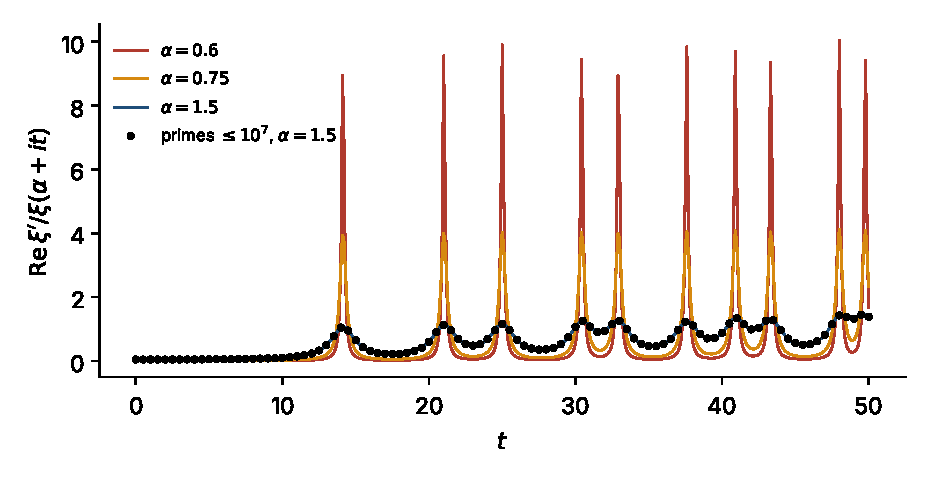
\includegraphics[width=\textwidth]{fig/v3/ch_ladder.pdf}
\caption{$\Re\,\xi'/\xi(\alpha+it)$ at $\alpha=0.6,0.75,1.5$. The peaks are Cauchy smoothed zeros; the width is $\alpha-\frac12$. Dots: the same quantity at $\alpha=1.5$ computed from the primes up to $10^7$. At $\alpha=0.75$, $t=20$ the exact value $0.255659$ agrees with the Poisson sum over the first thousand zeros, $0.255299$.}
% UNVERIFIED: the dots of this figure were not recomputed; the two printed values were (0.255659 and 0.255299).
\label{ct:fig:ladder}
\end{figure}

\section{Chebyshev 1850 and the Bondesson Gamma term}\label{ct:sec:gamma}

Chebyshev's identity \eqref{ct:eq:cheb} is a ratio of Gamma functions evaluated at integers:
\[
R(w)=\frac{\Gamma(1+w)\,\Gamma(1+w/30)}{\Gamma(1+w/2)\,\Gamma(1+w/3)\,\Gamma(1+w/5)}=\prod_k\Gamma(1+c_kw)^{\varepsilon_k}.
\]
The 1850 memoir compares $\sum u(n)\psi(x/n)$ with $\log R(x)$. In Thorin language it compares the L\'evy measure of the primes with the L\'evy measure of a signed product of Bondesson terms. A single Bondesson term is the function $e^{-\gamma\sqrt u}/\Gamma(1+\sqrt u)$ (Bondesson \cite{Bondesson}); its factorisation into a GGC is proved in Corollary~\ref{ct:cor:bondesson}.

\begin{theorem}[Chebyshev's Gamma ratio is a GGC]\label{ct:thm:chebggc}
For $w>0$,
\begin{multline}\label{ct:eq:Rlevy}
\log R(w)=\int_0^\infty\big(e^{-wy}+wy-1\big)\frac{g(y)}{y}\dd y,\\
g(y)=\sum_{n\ge1}u(n)e^{-ny}=(1-e^{-y})\sum_{n\ge1}U(n)e^{-ny}\ge0.
\end{multline}
Hence, with $r=\sqrt z$,
\begin{multline*}
\frac1{R(\sqrt{u})}=\exp\Big(-\int_0^\infty\log\Big(1+\frac uz\Big)t_C(z)\dd z\Big),\\
t_C(z)=\frac{1}{2\pi r}\sum_k\varepsilon_kc_k\,\Re\,\psi_\Gamma(1+ic_kr)\ge0,
\end{multline*}
so $u\mapsto1/R(\sqrt u)$ is the Laplace transform of a generalised gamma convolution with Thorin density $t_C$. Further,
\begin{multline*}
t_C(z)\sim\frac{A}{2\pi\sqrt{z}}\quad(z\to\infty),\\
t_C(z)\sim\frac{\zeta(3)\big(1-\tfrac18-\tfrac1{27}-\tfrac1{125}+\tfrac1{27000}\big)}{2\pi}\sqrt{z}\quad(z\to0).
\end{multline*}
\end{theorem}

\begin{proof}
Malmst\'en's formula gives $\log\Gamma(1+cw)=-\gamma cw+\int_0^\infty(e^{-wy}-1+wy)\frac{\dd y}{y(e^{y/c}-1)}$. Sum with signs $\varepsilon_k$: the terms $-\gamma c_kw$ cancel because $\sum\varepsilon_kc_k=0$, and $\sum_k\varepsilon_k(e^{y/c_k}-1)^{-1}=\sum_ne^{-ny}\sum_k\varepsilon_k[c_k^{-1}\mid n]=\sum_nu(n)e^{-ny}$ by Proposition~\ref{ct:prop:cheb1850}(i). Abel summation with $U(0)=0$ gives the second form of $g$, which is nonnegative because $U\in\{0,1\}$. The sine squared lemma with $x=y$ gives the Thorin representation with $t_C(z)=\frac{1}{2\pi r}\int_0^\infty(1-\cos ry)g(y)\dd y\ge0$. The closed form follows from $\int_0^\infty\frac{1-\cos ay}{e^{y/c}-1}\dd y=c\big(\Re\psi_\Gamma(1+iac)+\gamma\big)$, and again the $\gamma$ terms cancel. As $r\to\infty$, $\Re\psi_\Gamma(1+it)=\log t+O(t^{-2})$, so $2\pi rt_C\to\sum\varepsilon_kc_k\log(c_kr)=A$. As $r\to0$, $\Re\psi_\Gamma(1+it)+\gamma=\zeta(3)t^2+O(t^4)$, giving the behaviour at $0$.
\end{proof}

\begin{corollary}[explicit Thorin density for Bondesson's function]\label{ct:cor:bondesson}
For $u>0$,
\begin{multline*}
\frac{e^{-\gamma\sqrt u}}{\Gamma(1+\sqrt u)}=\exp\Big(-\int_0^\infty\log\Big(1+\frac{u}{z}\Big)t_B(z)\dd z\Big),\\
t_B(z)=\frac{\Re\,\psi_\Gamma\big(1+i\sqrt{z}\big)+\gamma}{2\pi\sqrt{z}}\ge0.
\end{multline*}
\end{corollary}
\begin{proof}
Take a single factor $c=1$ in the proof of Theorem~\ref{ct:thm:chebggc}: the L\'evy density is $1/(y(e^y-1))\ge0$ and the $\gamma$ term stays. Positivity is $\Re\psi_\Gamma(1+it)\ge\psi_\Gamma(1)=-\gamma$.
\end{proof}

\begin{table}[t]
\centering\small
\begin{tabular}{lcccc}
\toprule
$w$ & $\log\Gamma(1+w)+\gamma w$ & Thorin side & $\log R(w)$ & Thorin side\\
\midrule
$0.5$ & $0.167825594816$ & $0.167825594816$ & $0.0929944417683$ & $0.0929944417683$\\
$2$ & $1.84757851036$ & $1.84757851036$ & $0.880135656529$ & $0.880135656529$\\
$10$ & $20.8765692221$ & $20.8765692221$ & $7.28482091257$ & $7.28482091257$\\
\bottomrule
\end{tabular}
\caption{Numerical check of Corollary~\ref{ct:cor:bondesson} and Theorem~\ref{ct:thm:chebggc} (computed). The Thorin side integrates $\log(1+w^2/z)$ against $t_B$ and $t_C$. The two sides agree to the twelve digits printed.}
\label{ct:tab:bondesson}
\end{table}

\begin{figure}[t]
\centering
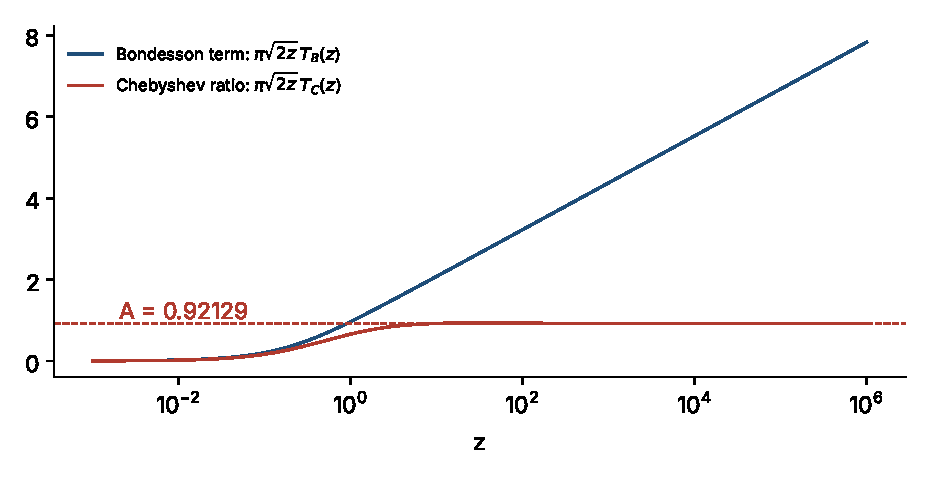
\includegraphics[width=\textwidth]{fig/v3/ch_bondesson.pdf}
% Redraw in z = r^2: the horizontal axis of this file is r^2/2. The plotted quantity is unchanged.
\caption{The normalised Thorin densities $2\pi r\,t_B$ and $2\pi r\,t_C$ against $r^2/2$. The Bondesson term grows like $\log r+\gamma$. In Chebyshev's ratio the logarithm cancels and the density approaches Chebyshev's constant $A$; at $r=10^3$ the value is $0.921294$ against $A=0.921292$. Both are nonnegative everywhere.}
\label{ct:fig:bondesson}
\end{figure}

\subsection{How the 1850 result matches the Bondesson term}
Three statements answer the question.

First, the Gamma factor of $\xi$ is a single Bondesson term at scale $c=\frac12$. Its Thorin density is $\frac{1}{4\pi r}\big(\Re\psi_\Gamma(1+ir/2)+\gamma\big)\sim\frac{\log(r/2)}{4\pi r}$. The atoms at the centre are $\gamma^2$ with counting density, by Riemann and von Mangoldt, $\frac{\log(r/2\pi)}{4\pi r}\dd z$. So the Bondesson term and the zeros have the same leading tail.

Second, Chebyshev's ratio is a signed product of five Bondesson terms with $\sum\varepsilon_kc_k=0$. That one condition cancels the pole of $\zeta$ ($P(1)=0$), cancels Euler's constant in the L\'evy representation, and cancels the $\log r$ in the Thorin tail. What survives is the constant $A$. Chebyshev's positivity $U\in\{0,1\}$ implies the positivity of $t_C$. The product is a signed product of Bondesson terms: four of the five factors enter with a minus sign, so it is a GGC only because the signs combine into a nonnegative floor combination.

Third, identity \eqref{ct:eq:cheb} transfers that GGC to the primes: the L\'evy measure of $\log R$ is $\sum u(n)e^{-ny}\dd y/y$ on the additive scale, while $\sum u(n)\psi(x/n)$ is the multiplicative convolution of the prime measure with the same weights. The Mellin transform links the two, $\int_0^\infty y^{s-1}g(y)\dd y=\Gamma(s)\zeta(s)P(s)$, in the way that Riemann's theta integral links $\Gamma(s/2)\zeta(s)$ to the Jacobi theta function.

The 1850 result works at level $\alpha=1$ and gives the two sided bound $A\le\psi(x)/x\le\frac65A$, not the limit. In the language of Theorem~\ref{ct:thm:dictionary} it gives the representation for $\alpha>1$ and no information about the strip. Its interest here is structural: a fully explicit, nonnegative Thorin density built from Gamma functions whose comparison with the primes is exact.

\begin{remark}[Sylvester and better weights]
% TODO: no bibliography entries for Sylvester 1881, 1892, and no source for the window [0.956,1.045]; authors to supply.
Sylvester (1881, 1892) used longer combinations with $\sum\varepsilon_kc_k=0$ to narrow the window to about $[0.956,1.045]$. Every such combination is a signed product of Bondesson terms. By the proof of Theorem~\ref{ct:thm:chebggc} it is a GGC in $u=w^2$ whenever its floor combination is nonnegative, and its Thorin tail constant is its Chebyshev constant. Nonnegativity is not necessary (Section~\ref{ct:sec:signed}); that nonnegativity of the running sums is not necessary is shown in Theorem~\ref{ct:thm:hier}, and a necessary and sufficient condition on the floor combination is Open problem~\ref{ct:op:signed}. Finding the best window is then an optimisation over GGCs with a positivity constraint, which is Open problem~\ref{ct:op:sylvester}.
\end{remark}

\begin{remark}[Ramanujan's ratio]
Ramanujan's 1919 proof of Bertrand's postulate uses the pair $T(x)-2T(x/2)$. Here $\sum\varepsilon_kc_k=0$ holds and the floor combination $\lfloor t\rfloor-2\lfloor t/2\rfloor$ takes values in $\{0,1\}$, so by Theorem~\ref{ct:thm:chebggc} the reciprocal of $\Gamma(1+\sqrt u)/\Gamma(1+\sqrt u/2)^2$ is a GGC with tail constant $\log2$.
\end{remark}

\section{Yamazato's integer part split}\label{ct:sec:yamazato}

Write the Laplace exponent of a GGC as $\int\log(1+\lambda/z)\,\mu(\dd z)$ and let $F(z)=\mu((0,z])$ (we keep $U$ for Chebyshev's floor combination). Integration by parts gives the L\'evy density
\[
\nu(y)=\frac1y\int_0^\infty e^{-yz}\mu(\dd z)=\int_0^\infty e^{-yz}F(z)\dd z .
\]
% TODO: no bibliography entries for the argument of Yamazato in the form Simon uses for stable laws; authors to supply.
The split below is an adaptation of an argument of Yamazato, in the form Simon uses for stable laws. The theorem of \cite{Yamazato78} is about unimodality in class $L$ and is a different result, so we give the short proof. 
\begin{lemma}[integer part split]\label{ct:lem:split}
Split $F=[F]+\{F\}$. Let $\kappa_n=\inf\{z:F(z)\ge n\}$. A GGC with Thorin distribution function $F$ is the independent sum of $\sum_n\mathrm{Exp}(\kappa_n)$ and a mixture of exponentials.
\end{lemma}
\begin{proof}
The integer part jumps by one at $\kappa_n$ and contributes $\sum_n e^{-y\kappa_n}/y$ to $\nu$, the L\'evy density of $\sum_n\mathrm{Exp}(\kappa_n)$. The fractional part satisfies $0\le\{F\}\le1$, so by Steutel's criterion \cite{Steutel67} $\int e^{-yz}\{F(z)\}\dd z$ is the L\'evy density of a mixture of exponentials.
\end{proof}

Gamma factorisations are the case $\{F\}=0$: $\Gamma(1+w)e^{\gamma w}=\prod_n(1+w/n)^{-1}e^{w/n}$ has $F(z)=\lfloor z\rfloor$. In Chebyshev's ratio each factor $\Gamma(1+c_kw)$ has Thorin distribution $\lfloor c_kz\rfloor=c_kz-\{c_kz\}$. The linear parts are Stirling's terms. They cancel because $\sum\varepsilon_kc_k=0$, and what is left is a pure fractional part:
\[
U(z)=\sum_k\varepsilon_k\lfloor c_kz\rfloor=-\sum_k\varepsilon_k\{c_kz\}\in\{0,1\}.
\]

\begin{theorem}[Chebyshev 1850 in Yamazato form]\label{ct:thm:chebME}
Let $A=0.92129\ldots$ and $R(w)=\prod_k\Gamma(1+c_kw)^{\varepsilon_k}$. Then
\[
e^{-Aw}R(w)=\mathbb E\,e^{-wX_C},
\]
where $X_C\ge0$ is infinitely divisible with L\'evy density $\nu_C(y)=\int_0^\infty e^{-yz}U(z)\dd z=\frac1y\sum_nu(n)e^{-ny}$. Since $0\le U\le1$, $X_C$ is a mixture of exponentials, and since $\nu_C(y)\sim\frac{1}{2y}$ as $y\to0$ it has no atom at zero. Its Steutel function is Chebyshev's floor combination.
\end{theorem}
\begin{proof}
From \eqref{ct:eq:Rlevy}, $\log R(w)=\int(e^{-wy}-1)\nu_C(y)\dd y+w\int y\nu_C(y)\dd y$, and $\int_0^\infty y\nu_C(y)\dd y=\int_0^\infty g(y)\dd y=\sum_nu(n)/n=A$ (Abel summation, using $P(1)=0$ and $P'(1)=A$). The representation $g(y)=y\int e^{-yz}U(z)\dd z$ is integration by parts. As $y\to0$, $g(y)\to$ the mean of $U$ over a period, which is $\tfrac12$.
\end{proof}

Numerically (computed) $\log R(w)-Aw$ and $-\int(1-e^{-wy})\nu_C(y)\dd y$ agree to all twelve printed digits at $w=0.5,2,10,50$, for example $-1.92809931677$ at $w=10$.

The theorem expresses the Chebyshev error through the Gamma term. Since $\log\lfloor y\rfloor!=\log\Gamma(1+y)-\{y\}\log y+O(1/y)$, identity \eqref{ct:eq:cheb} and Stirling give
\begin{equation}\label{ct:eq:uweighted}
\sum_{n\le x}u(n)\,\big(\psi(x/n)-x/n\big)=\log\mathbb E\,e^{-xX_C}+U(x)\log x+O(1)=\Big(U(x)-\frac12\Big)\log x+O(1).
\end{equation}
The $-\frac12\log x$ is the ME law $X_C$, that is, the Gamma term, and the $U(x)\log x$ is Yamazato's fractional part. So Chebyshev's weighted error swings between $-\frac12\log x$ and $+\frac12\log x$ according to the fractional parts of $x/2,x/3,x/5,x/30$. On $[10^2,10^7]$, at half integer $x$, the remainder in \eqref{ct:eq:uweighted} lies in $[-3.08,1.25]$ (computed). The range depends on the fractional part of $x$: at integer $x$ it is $[-2.62,1.71]$.

\begin{figure}[t]
\centering
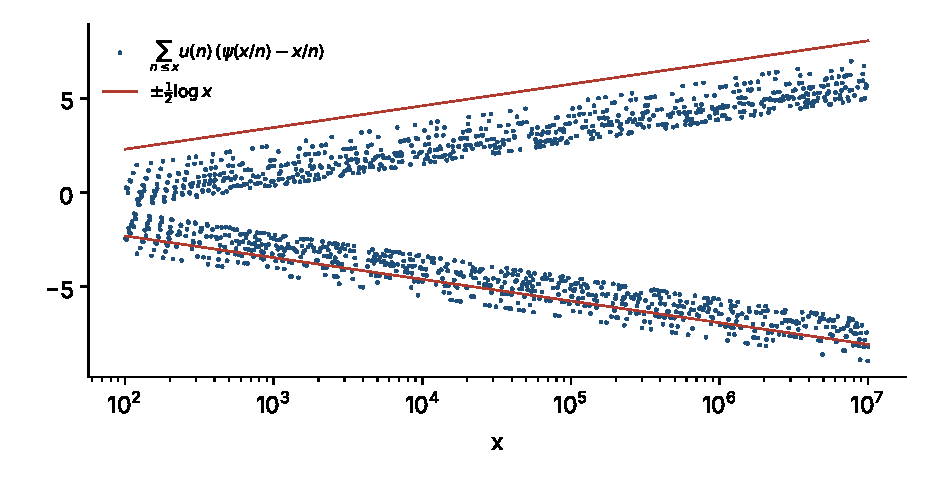
\includegraphics[width=\textwidth]{fig/v3/ch_uweighted.pdf}
\caption{Chebyshev's weighted error $\sum_{n\le x}u(n)(\psi(x/n)-x/n)$ against $\pm\frac12\log x$. The two branches are $U(x)=1$ and $U(x)=0$.}
\label{ct:fig:uweighted}
\end{figure}

\subsection{The reciprocal Xi function}
By Theorem~\ref{ct:thm:dictionary}, the Thorin distribution function at level $\alpha$ is, with $r=\sqrt z$,
\[
F_\alpha(z)=\int_0^zt_\alpha=\frac1\pi\int_0^r\big(v_\alpha(s)-b_\alpha\big)\dd s=\frac1\pi\Big(\arg\xi(\alpha+ir)-r\,b_\alpha\Big),
\]
the argument taken continuously from $\arg\xi(\alpha)=0$ (derived above for $\alpha>1$ and, where $t_\alpha\ge0$, by Theorem~\ref{thm:poisson} for $\alpha>\Theta$). So the Thorin distribution function is a phase. Writing $\arg\xi=\arg\big(\tfrac12s(s-1)\pi^{-s/2}\Gamma(s/2)\big)+\arg\zeta$, the first piece is the Gamma phase and the second is the prime phase, $\arg\zeta(\alpha+ir)=-\int_0^\infty e^{-\alpha u}\sin(ru)\,\dd\psi(e^u)/u$ for $\alpha>1$.

\begin{proposition}[Yamazato split of the reciprocal Xi]\label{ct:prop:yamxi}
For $\alpha>\Theta$ with $t_\alpha\ge0$,
\[
\frac{\xi(\alpha)}{\xi(\alpha+\sqrt{u})}\,e^{\sqrt{u}\,b_\alpha}=\prod_{n\ge1}\Big(1+\frac{u}{\kappa_{\alpha,n}}\Big)^{-1}\cdot\mathbb E\,e^{-uY_\alpha},
\]
where $\kappa_{\alpha,n}=r_{\alpha,n}^2$ with $F_\alpha(r_{\alpha,n}^2)=n$, and $Y_\alpha$ is a mixture of exponentials with Steutel function $\{F_\alpha\}$. At the centre, under RH, $\{F_{1/2}\}=0$ and
\[
\frac{\xi(\frac12)}{\xi(\frac12+w)}=\prod_{\gamma>0}\Big(1+\frac{w^2}{\gamma^2}\Big)^{-1},
\]
a pure exponential series with rates $\gamma^2$.
\end{proposition}
\begin{proof}
Lemma~\ref{ct:lem:split} with the Thorin distribution function $F_\alpha$ and \eqref{ct:eq:thorinform}, which for $\Theta<\alpha\le1$ follows from Theorem~\ref{thm:poisson} since $\frac1\pi\int_0^\infty\log(1+u/r^2)\,b_\alpha\dd r=b_\alpha\sqrt u$. At the centre under RH, $F_{1/2}=N(r)$ is integer valued.
\end{proof}

The product at the centre was checked (computed) against $2000$ zeros plus the Riemann and von Mangoldt tail: at $w=1$ both sides are $0.97718$ and at $w=3$ both are $0.81345$. The integer and half integer crossings of $F_\alpha$ behave very differently (Table~\ref{ct:tab:yam}, Figure~\ref{ct:fig:yam}), as the numbers below (computed from $8000$ zeros) show.
\begin{itemize}
\item The half integer crossings $F_\alpha=n-\frac12$ are the zeros: at $\alpha=0.52$ they reproduce $\gamma_1,\ldots,\gamma_{10}$ to within $0.001$, and at $\alpha=0.75$ to within $0.13$. Statistically, $\{F_\alpha\}$ passes through $\frac12$ at each zero, as a Cauchy smoothed step does, at levels near the line and at low height; at $\alpha=1$ the compensator drift moves the crossings (Section~\ref{ct:sec:yamcheb}).
\item The integer crossings, which are Yamazato's exponential rates (as $r_{\alpha,n}$), interlace with the zeros and hardly move with $\alpha$: $18.544,\allowbreak\ 23.688,\allowbreak\ 29.015,\allowbreak\ 32.165,\allowbreak\ 36.660,\ldots$ at $\alpha=0.55$ and $18.563,\allowbreak\ 23.730,\allowbreak\ 29.058,\allowbreak\ 32.244,\allowbreak\ 36.735,\ldots$ at $\alpha=1$. The first rate at $\alpha=1$ is $\kappa_{1,1}=r_{1,1}^2\approx344.6$.
\end{itemize}

\begin{conjecture}[the limit of the Yamazato rates]\label{ct:conj:canonical}
Assume RH and simple zeros. As $\alpha\downarrow\frac12$, $r_{\alpha,n}$ converges to the critical point $r^*_n\in(\gamma_n,\gamma_{n+1})$ of the genus one canonical product
\[
\mathcal E(r)=\prod_{\gamma>0}\Big(1-\frac{r^2}{\gamma^2}\Big)e^{r^2/\gamma^2}=\frac{\Xi(r)}{\Xi(0)}\,e^{qr^2/2},\qquad
q=\Big(\frac{\xi'}{\xi}\Big)'(\tfrac12)=\sum_{\gamma>0}\frac2{\gamma^2}=0.0462100,
\]
where $\Xi(r)=\xi(\frac12+ir)$.
\end{conjecture}
\begin{proof}[Heuristic derivation]
For $\alpha=\frac12+\epsilon$ and $r$ between zeros, $\arg\xi(\alpha+ir)=\pi N(r)-\epsilon\sum_\rho(r-\gamma)^{-1}+O(\epsilon^2)$ and $b_\alpha=\epsilon q+O(\epsilon^2)$. So $F_\alpha=N(r)-\frac\epsilon\pi\big(\frac{\Xi'}{\Xi}(r)+qr\big)+O(\epsilon^2)$, and $F_\alpha=n$ in $(\gamma_n,\gamma_{n+1})$ would force $\frac{\Xi'}{\Xi}(r)+qr=0$, which is $\mathcal E'(r)=0$. Between consecutive zeros $\mathcal E'/\mathcal E$ runs from $+\infty$ to $-\infty$, so a root exists. It is unique where $(\mathcal E'/\mathcal E)'=q-\sum_\rho(r-\gamma)^{-2}<0$, which holds on every gap of length $L<\sqrt{8/q}=13.158$, since the two zeros nearest to $r$ already give $\sum_\rho(r-\gamma)^{-2}\ge8/L^2$; by Lemma~\ref{yo:lem:gap} every gap is at most $6.8874$. The step that is not proved is the uniformity in $r$ of the expansion in $\epsilon$, which is why we state a conjecture.
\end{proof}

The critical points computed directly from $\Xi$ (computed) are $18.5441$, $23.6880$, $29.0144$, $32.1642$, $36.6589$, $40.1353$, $42.7567$, $47.2389$, $49.3101$, $52.4574$, which agree with the $\alpha=0.55$ crossings to within $0.002$. They are not the critical points of $\Xi$ itself ($15.59, 22.10, 26.27,\ldots$), and they are not Gram points ($17.85, 23.17, 27.67,\ldots$). The Gaussian factor $e^{qr^2/2}$ is the compensator $w\,b_\alpha$ of Theorem~\ref{ct:thm:dictionary} in the limit.
% UNVERIFIED: the critical points of Xi itself and the Gram points were not checked by the verification (the alpha = 0.55 and alpha = 1 lists were).

\begin{table}[t]
\centering\small
\begin{tabular}{rrrrr}
\toprule
$n$ & $\gamma_n$ & $F_{0.52}=n-\frac12$ & $F_{0.55}=n$ & $\mathcal E'=0$\\
\midrule
1 & 14.135 & 14.135 & 18.544 & 18.544\\
2 & 21.022 & 21.022 & 23.688 & 23.688\\
3 & 25.011 & 25.011 & 29.015 & 29.014\\
4 & 30.425 & 30.425 & 32.165 & 32.164\\
5 & 32.935 & 32.935 & 36.660 & 36.659\\
6 & 37.586 & 37.587 & 40.136 & 40.135\\
7 & 40.919 & 40.919 & 42.758 & 42.757\\
8 & 43.327 & 43.328 & 47.240 & 47.239\\
9 & 48.005 & 48.006 & 49.312 & 49.310\\
10 & 49.774 & 49.775 & 52.459 & 52.457\\
\bottomrule
\end{tabular}
\caption{Zeros, half integer crossings of the Thorin distribution function, Yamazato's integer crossings, and critical points of the canonical product (computed; entries agree with an independent recomputation to the printed digits, up to $0.0006$).}
\label{ct:tab:yam}
\end{table}

\begin{figure}[t]
\centering
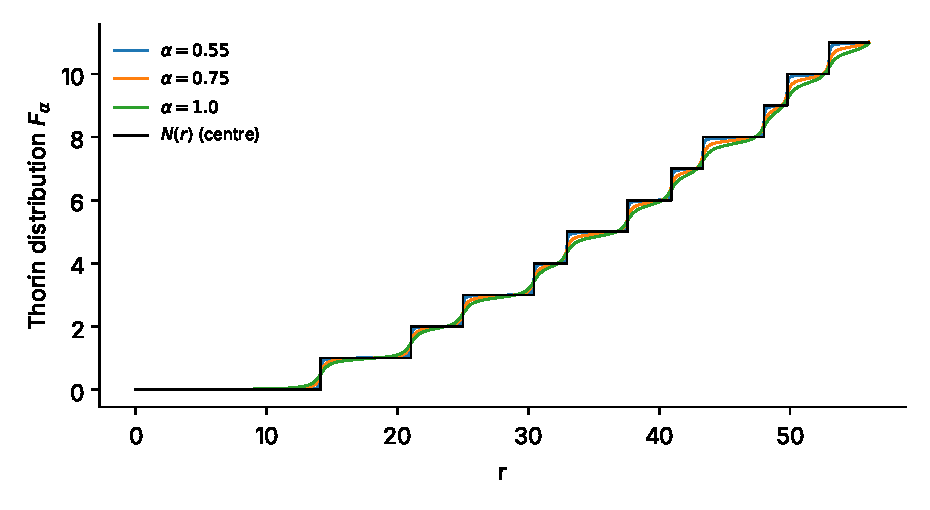
\includegraphics[width=\textwidth]{fig/v3/ch_yamazato.pdf}
\caption{Thorin distribution functions $F_\alpha$ at three levels against the counting function $N(r)$ at the centre. Integer crossings give Yamazato's exponential rates; half integer crossings give the zeros.}
\label{ct:fig:yam}
\end{figure}

\begin{remark}[what the split buys]
The exponential series is an explicit Gamma type factorisation whose rates are computable from $\arg\xi$ along a vertical line. The ME remainder has Steutel function $\{F_\alpha\}$ between $0$ and $1$, so its positivity is automatic. What remains of the difficulty of the descent is the requirement that $F_\alpha$ be nondecreasing, which is $t_\alpha\ge0$. Chebyshev's ratio is the case where the integer part is empty and the fractional part is everything, and that is why its positivity reduces to $U\in\{0,1\}$.
\end{remark}

\section{Rung one, the ladder and what is added here}\label{ct:sec:rung}

The note proves $v_1(r)\ge b_1$ for all real $r$ by convexity, a floating point grid and zero counting. This is known and is in Volume I. We state what is where.
\begin{itemize}
\item Level one. $v_1(r)>v_1(0)=b_1=1+\frac\gamma2-\frac12\log4\pi=0.0230957\ldots$ for every $r\ne0$, with no hypothesis (Proposition~\ref{bp:prop:v1min}, which uses the zeros below height $2000$ in ball arithmetic and the bounds of \cite{HSW22} above); the same constant $b_1/\pi$ appears in Theorem~\ref{cx:thm:globalmin}. Consequently $T_1\stackrel d=S+T_1^\circ$ with $T_1^\circ$ a GGC, and the Yamazato split of Section~\ref{ct:sec:yamazato} applies to it.
\item Every level $\alpha\ge1$ (Proposition~\ref{bp:prop:valpha}); the minimum of $\Re\frac{\xi'}{\xi}(\alpha+ir)$ at $r=0$ is due to Lagarias \cite{Lagarias} for $\alpha>10$ and to Garunk\v{s}tis \cite{Garunkstis02} for $\alpha>1$, and by letting $\alpha\downarrow1$ for $\alpha=1$ (the unconditional statement, without the strict inequality). Volume I adds the strict inequality.
\item Levels $\frac12<\alpha<1$. Under RH, $v_\alpha(r)\ge b_\alpha$ is due to Lagarias \cite{Lagarias}, in strict form Theorem~\ref{thm:dbeta:minall}, which also proves it unconditionally for every $\alpha\in(\frac12,7.35]$ and $0<|r|\le3\cdot10^{12}-1.21$ from the verification of RH to that height \cite{PT21}.
\item The equivalence of RH with the positivity of every $t_\alpha$, $\alpha>\frac12$, is Theorem~\ref{thm:dbeta:minall}(vi) and Theorem~\ref{thm:poisson}. On each line $t_\alpha\ge0$ implies Lagarias's positivity, since $b_\alpha>0$. We do not claim the converse on a line.
\end{itemize}

We add two computations, both for $\alpha=1$ and both independent of the argument of Volume I.

\paragraph{Range II, certified.} Range I is the convexity step, $0\le r\le\gamma_1-1/\sqrt3=13.557375$, where $v_1(r)>b_1$ because every Cauchy kernel $P_a(\gamma\pm r)$ is convex in $r$ for $|r\mp\gamma|>a/\sqrt3$, hence on $0\le r\le\gamma_1-1/\sqrt3$ (the convexity step of Proposition~\ref{bp:prop:v1min}). On the remaining bounded range $13.557375\le r\le2000$ we computed $v_1(r)-b_1$ in ball arithmetic directly from $\zeta$ and the digamma function with $64$ bit balls, with $r$ a ball on each cell and adaptive bisection (floor width $10^{-7}$). No list of zeros is used. Over $179{,}072$ cells there were no failures, and $v_1(r)-b_1>0.0900$ on the whole range (certified). The true minimum is $0.0901596$ at $r=17.4928$, between $\gamma_1$ and $\gamma_2$; the next local minima are $0.167$ near $27.66$, $0.432$ near $109.04$ and $0.867$ near $526.43$ (computed).

\paragraph{Range III with the bound of Hasanalizade, Shen and Wong.} For $r\ge2000$ take the window $|\gamma-r|\le H=8.75$. Each zero pays at least $\frac1{4(1+H^2)}$ in $v_1$ (a zero off the line pays together with its mirror image; Volume I has the better bound of one half per zero, and the weaker one is the one for which our margin was computed), and the number of zeros in the window is at least $K(r)$, obtained from the Stirling expansion of $\theta'$ and the bound $|S(T)|\le0.1095\log T+0.2042\log\log T+3.0305$ of \cite{HSW22} (Trudgian's bound is not used, because its proof is incomplete \cite{BMOR21,HSW22}). At $r=2000$ the margin $K(r)/(4(1+H^2))-b_1$ is $0.00103>0$ with this bound, increasing in $r$ (computed, floating point; we checked that $K$ increases from $2000$ to $10^{12}$). The inequality for all $r\ge2000$ follows from the monotonicity of $K$, whose derivative is at least $\big(\frac H\pi\frac{r-H}{r+H}-0.219-0.4084/\log(r-H)\big)/(r-H)>0$ up to the Stirling remainder.

The note's table of margins for $1\le\alpha\le9$ was recomputed and its second range column differs from our values by up to $0.0013$ for $\alpha\ge4$; we do not print it. All margins are positive in our recomputation, and Proposition~\ref{bp:prop:valpha} is the statement to cite.

\section{The statistician's view of $\psi(x)-x$}\label{ct:sec:stat}

\subsection{Variance and the Thorin measure at the centre}
Under RH the normalised error $Z(u)=e^{-u/2}E(u)\approx-2\sum_{\gamma>0}\cos(\gamma u-\arg\rho)/|\rho|$ is an almost periodic function of $u=\log x$.

\begin{remark}[Cram\'er 1922 in Thorin form]\label{ct:rem:cramer}
Assume RH and simple zeros. Then by Proposition~\ref{wt:prop:energy} (Cram\'er \cite{Cramer})
\begin{multline*}
\lim_{X\to\infty}\frac1{\log X}\int_1^{X}\Big(\frac{\psi(x)-x}{\sqrt x}\Big)^2\frac{\dd x}{x}\\=\sum_\rho\frac{1}{|\rho|^2}=2\int_0^\infty\frac{U_{\rm RH}(\dd z)}{z+\frac14}=2+\gamma-\log4\pi=0.0461914\ldots,
\end{multline*}
where $U_{\rm RH}=\sum_{\gamma>0}\delta_{\gamma^2}$ is the Thorin measure at the centre. Indeed $|\rho|^2=\frac14+\gamma^2$ and each $\gamma>0$ appears twice in $\sum_\rho$. So the variance of Chebyshev's error is the Stieltjes transform of the centre Thorin measure at $\frac14$, a quantity a statistician can estimate from the primes. With the first thousand zeros and the Riemann and von Mangoldt tail we get $0.046192$ (computed). The constant $\sum_\rho|\rho|^{-2}$ is different from $q=\sum_{\rho}\gamma^{-2}$ in Conjecture~\ref{ct:conj:canonical}.
\end{remark}

From primes up to $10^7$, sampling $x$ uniformly on the log scale in $[10^2,10^7]$, the second moment of $(\psi(x)-x)/\sqrt x$ is $0.0488$ and the mean is $-0.030$ for real $x$ (computed); for integer $x$ the values are $0.0475$ and $-0.021$. They approach $0.0462$ only slowly: on $[10^3,10^7]$ the real $x$ values are $0.0470$ and $-0.0106$. The maximum of $|\psi(x)-x|/\sqrt x$ on $[10^2,10^7]$ is $0.803$ over real $x$ ($0.7955$ on a grid of $10^4$ points).

\begin{remark}[the mean of $\theta$]
For $\theta$ instead of $\psi$ the same computation gives mean $-1$, because $\psi(x)-\theta(x)=\sqrt x+O(x^{1/3})$. The prime squares are a compensator, the same effect that biases Chebyshev's race modulo $4$ and P\'olya's Liouville sum. On $[10^2,10^7]$ we observe mean $-1.20$ and variance $0.0568$ for real $x$ (computed); the excess over $-1$ is the $x^{1/3}$ term, which decays slowly on the log scale.
\end{remark}

\subsection{Zeros from primes: the periodogram}
The line spectrum of $Z$ sits at the ordinates $\gamma$, the square roots of the atoms of the centre Thorin measure, so the periodogram of $Z$ estimates the ordinates. Figure~\ref{ct:fig:periodogram} uses a Hann taper on $u\in[\log10^2,\log10^7]$, a window of length $11.5$ and resolution about $2\pi/11.5\approx0.55$. The peaks found are (computed)
\[
14.14,\ 21.03,\ 25.02,\ 30.43,\ 32.95,\ 37.59,\ 40.92,\ 43.34,\ 48.00,\ 49.79,\ 52.98,\ 56.46,
\]
% UNVERIFIED: the peak list was not recomputed.
against the true ordinates $14.13$, $21.02$, $25.01$, $30.42$, $32.94$, $37.59$, $40.92$, $43.33$, $48.01$, $49.77$, $52.97$, $56.45$ (rounded to two decimals; checked against the zeros). Statistically this is line spectrum estimation. The resolution limit is of order $2\pi/\log X$, so on this heuristic one needs $\log X\gtrsim2\pi/\Delta$ to separate zeros at distance $\Delta$.

\begin{figure}[t]
\centering
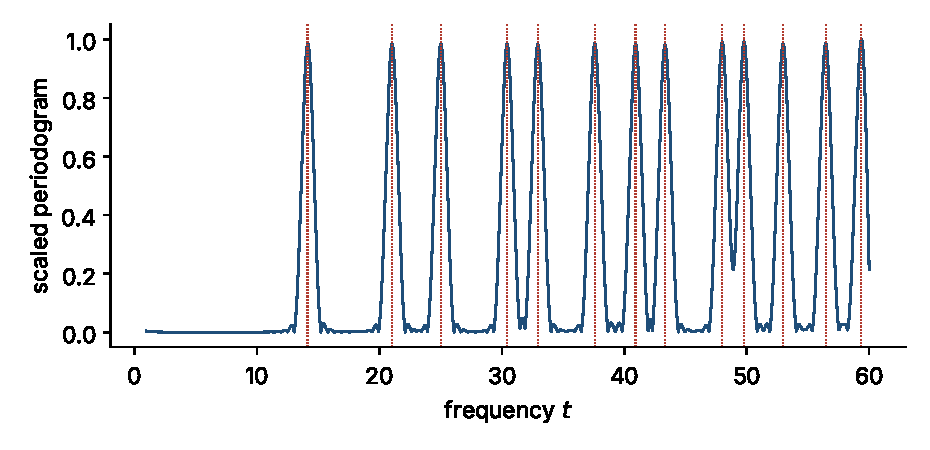
\includegraphics[width=\textwidth]{fig/v3/ch_periodogram.pdf}
% UNVERIFIED
\caption{Scaled periodogram $t\,|\hat Z(t)|$ of the normalised Chebyshev error from primes up to $10^7$. Dotted lines: ordinates of the zeros.}
\label{ct:fig:periodogram}
\end{figure}

\subsection{The limiting distribution and extremes (heuristic)}
If the ordinates are linearly independent over $\mathbb Q$ (Ingham's hypothesis LI \cite{Ingham42}), then for $u$ uniform on $[0,U]$ the law of $Z(u)$ converges to that of $\sum_{\gamma>0}\frac{2}{|\rho|}\cos V_\gamma$ with independent uniform phases $V_\gamma$, the Wintner law (Wintner 1935%
% TODO: no bibliography key for Wintner 1935; authors to supply
, who proved the existence of the limit under RH; the independent phase form needs LI). Its characteristic function is $\prod_{\gamma>0}J_0(2t/|\rho|)$. Each factor is a planar rotor. This is a law of $Z$ in $u=\log x$; it is a different object from the value distribution in $t$ of the prime side transform at fixed $\alpha$ (Kershner and Wintner \cite{KershnerWintner37}). Figure~\ref{ct:fig:wintner} compares the data with a simulation of the rotor model using the first thousand zeros.

\begin{figure}[t]
\centering
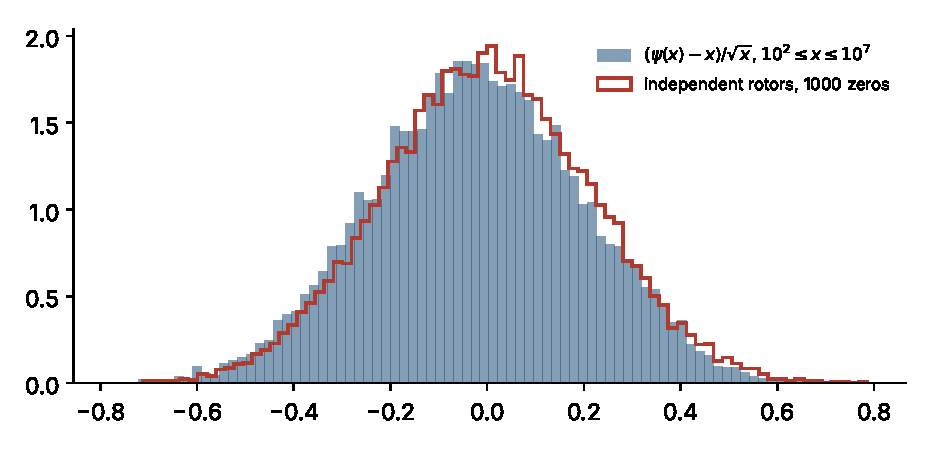
\includegraphics[width=\textwidth]{fig/v3/ch_wintner.pdf}
% UNVERIFIED
\caption{Distribution of $(\psi(x)-x)/\sqrt x$ for $x$ uniform on the log scale in $[10^2,10^7]$, against the independent rotor model with amplitudes $2/|\rho|$.}
\label{ct:fig:wintner}
\end{figure}

The rotor law has double exponential tails, $\exp(-e^{c_2\sqrt V})\le P(Z>V)\le\exp(-e^{c_1\sqrt V})$ (Montgomery 1980%
% TODO: no bibliography key for Montgomery 1980; authors to supply
; Rubinstein and Sarnak \cite{RubinsteinSarnak94} in the race setting). The cumulant function is $K(\theta)=\log\mathbb Ee^{\theta Z}=\sum_{\gamma>0}\log I_0(2\theta/|\rho|)$, and with the Riemann and von Mangoldt density of ordinates, $K(\theta)=\frac{\theta}{2\pi}\log^2\theta\,(1+o(1))$ as $\theta\to\infty$ (the sum $\sum_{\gamma<2\theta}2\theta/\gamma$ by partial summation against $N(T)$; the zeros above $2\theta$ contribute $O(\theta\log\theta)$ since $\log I_0(x)\le x^2/4$). A saddlepoint argument (not carried out here) then gives $\log\big(-\log P(Z>V)\big)=\sqrt{2\pi V}(1+o(1))$. The extreme value step is a heuristic: on $[0,U]$ there are about $U$ effectively independent windows, so the running maximum reaches $V$ when $\sqrt{2\pi V}\approx\log\log U$, that is $V\approx\frac1{2\pi}(\log\log\log x)^2$. This is the scale and the constant $\frac1{2\pi}$ of Montgomery's conjecture, which Montgomery obtained from the same independent phase model. Littlewood's theorem proves records of size $\log\log\log x$. What is missing is the transfer from the independent model to the almost periodic function $Z(u)$, which needs a quantitative Kronecker theorem for the ordinates (LI is a hypothesis throughout).

Over the range reachable here the slope of $\log(-\log P)$ against $\sqrt{2\pi V}$ computed with the $1545$ zeros and the density beyond is $1.34$ rather than $1$ (Figure~\ref{ct:fig:p4}), because the $\log\log$ corrections are large. The crude window count predicts a record of $0.42$ for $x\le10^7$ against the observed $0.803$, so the number of effective windows is larger than the count and the prediction is a leading order statement only.
% UNVERIFIED: slope 1.34 and the 0.42 were not recomputed.

\begin{figure}[t]
\centering
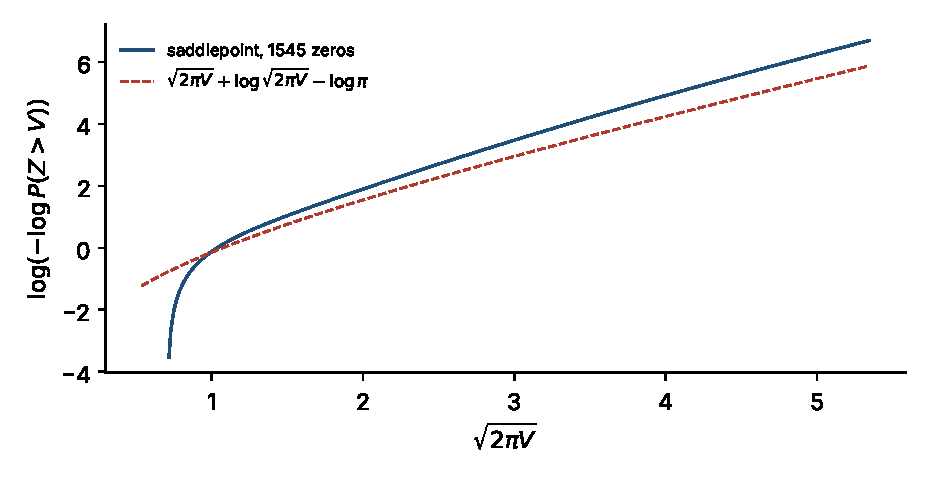
\includegraphics[width=\textwidth]{fig/v3/fig_p4_tail.pdf}
% UNVERIFIED
\caption{Saddlepoint tail of the rotor law: $\log(-\log P(Z>V))$ against $\sqrt{2\pi V}$, with the asymptotic form.}
\label{ct:fig:p4}
\end{figure}

\section{Signed products of Gamma functions}\label{ct:sec:signed}

\begin{theorem}\label{ct:thm:runningsums}
Let $R(w)=\prod_d\Gamma(1+w/d)^{a_d}$ with $\sum_da_d/d=0$, let $U(t)=\sum_da_d\lfloor t/d\rfloor$, which has period $L=\mathrm{lcm}\{d\}$, and let $V(k)=\sum_{j=1}^kU(j)$. If $V(k)\ge0$ for $1\le k\le L$, then $1/R(\sqrt u)$ is the Laplace transform of a GGC.
\end{theorem}
\begin{proof}
As in Theorem~\ref{ct:thm:chebggc}, $2\pi rt(z)=\sum_nu(n)\varphi_r(n)$ with $\varphi_r(x)=r^2/(x(x^2+r^2))$, and Abel summation gives $\sum_nU(n)\Delta\varphi_r(n)$ with $\Delta\varphi_r(n)=\varphi_r(n)-\varphi_r(n+1)$. Writing $p(x)=x^3+r^2x$, $\varphi_r=r^2/p$ and $2p'^2-pp''=12x^4+6r^2x^2+2r^4>0$, so $\varphi_r$ is convex and $\Delta\varphi_r$ is decreasing. Grouping by residues modulo $L$, $\sum_nU(n)\Delta\varphi_r(n)=\sum_{j=1}^LU(j)W(j)$ with $W(j)=\sum_{m\ge0}\Delta\varphi_r(j+mL)$ decreasing in $j$, and a second Abel summation gives $V(L)W(L)+\sum_{k<L}V(k)(W(k)-W(k+1))\ge0$.
\end{proof}

So nonnegativity of the floor combination is sufficient but not necessary, and nonnegativity of its running sums is sufficient but not necessary either (Theorem~\ref{ct:thm:hier}). The smallest example is
\[
R(w)=\frac{\Gamma(1+w)\,\Gamma(1+w/6)^2}{\Gamma(1+w/2)^2\,\Gamma(1+w/3)},
\]
with $U=(1,0,0,-1,0,0)$ and $V=(1,1,1,0,0,0)$ over one period. It is a GGC with tail constant $\frac23\log2$ even though $U$ takes the value $-1$ (proved; the constants were rechecked). Among the $225$ products with $d\le30$, at most five factors and exponents in $\{\pm1,\pm2\}$ that have positive tail constant, all $225$ have $t\ge0$ on a grid of $2200$ values of $r$, and $87$ of them have $U<0$ somewhere; every one of these $87$ that we inspected has $V\ge0$ (computed%
% TODO: state how many of the 87 were inspected
).
% UNVERIFIED: the search over 225 products and the constants 0.85228 and 0.78036 were not recomputed.
Within the same search space the largest Chebyshev constant with $0\le U\le1$ is Chebyshev's own $A=0.92129$; the next are $0.85228$ (divisors $1,2,3,4,12$) and $0.78036$ (computed). % TODO: Diamond and Erd\H{o}s (1980) has no bibliography entry; the authors must supply one or cut the sentence.
Diamond and Erd\H{o}s (1980) showed that Chebyshev type combinations can bring both constants arbitrarily close to $1$, although their proof uses the prime number theorem. Theorem~\ref{ct:thm:runningsums} enlarges the class of admissible combinations that are GGCs, which is the setting in which the optimisation should be posed.

\section{Zeros from primes by positive deconvolution}\label{ct:sec:deconv}

At level $\alpha=1.5$ the data $v_{1.5}(r)=\Re\frac{\xi'}{\xi}(1.5+ir)$ can be computed from the primes alone: the prime sum $\sum\Lambda(n)n^{-1.5}\cos(r\log n)$ converges absolutely, and truncation at $n\le10^6$ costs at most $0.0031$ at $r=0$ and far less elsewhere (computed), against a direct evaluation to $0.002$ (the tail beyond $10^6$ is about $2\cdot10^{-3}$ at $r=0$, so the two agree within the truncation bound).
% UNVERIFIED: the truncation bound 0.0031 was not recomputed.
 Under RH, $v_{1.5}$ is a Cauchy smoothing of the zero spectrum with width $a=1$:
\[
v_{1.5}(r)=\sum_{\gamma>0}\Big(\frac{1}{1+(r-\gamma)^2}+\frac{1}{1+(r+\gamma)^2}\Big).
\]
We treat this as a deconvolution problem in two stages, as in the Bayesian deconvolution of Volume II (Section~\ref{lo:sec:gbc}) and the EM methods of \cite{Richardson72,Lucy74,VardiLee93} (see also \cite{PadillaPolsonScott18}).
\begin{enumerate}
\item An EM step for a nonnegative measure on a grid of step $0.05$ on $[0,210]$, with no assumption on the number or location of atoms. After $4000$ iterations the misfit is $1.2\%$ of the data range and the estimate has $78$ clear atoms below $200$ (Figure~\ref{ct:fig:p3}).
\item A line fit in which each atom carries its own position $\gamma_k$, width $a_k$ and mass $m_k$, so that $\beta_k=1.5-a_k$ estimates the real part of the zero and $m_k$ its multiplicity. Zeros above $200$ enter only through the smooth Riemann and von Mangoldt density $\frac1{2\pi}\log\frac u{2\pi}$, so no zero location is used.
\end{enumerate}
Masses must be whole numbers, which gives a model selection rule: an atom whose fitted mass is near $2$ is two zeros. The rule fires twice, at $169.5$ and $185.2$, both pairs closer than the smoothing width. After splitting, the fit below $180$ gives exactly $69$ zeros, matching $N(180)=69$, with
\[
\max_k|\hat\gamma_k-\gamma_k|=0.0031,\qquad0.4983\le\hat\beta_k\le0.5042,\qquad0.989\le\hat m_k\le1.010 .
\]
(All computed.) % UNVERIFIED except N(180)=69 and N(200)=79.
This is not a test of RH. An off line pair $\beta=\frac12\pm\delta$ at one ordinate contributes kernels of widths $1-\delta$ and $1+\delta$ with $P_{1-\delta}+P_{1+\delta}=2P_1+O(\delta^2)$, so to first order it is indistinguishable from two zeros on the line, which is exactly what the integer mass rule reports. The zeros below $180$ are known to lie on the line anyway. The resolution is set by the width $\alpha-\frac12$: pairs closer than about $0.8$ (not verified) merge at $\alpha=1.5$ and are recovered only through the integer mass rule. Lowering $\alpha$ sharpens the kernel but slows the convergence of the prime sum as $X^{1-\alpha}$.

\begin{figure}[t]
\centering
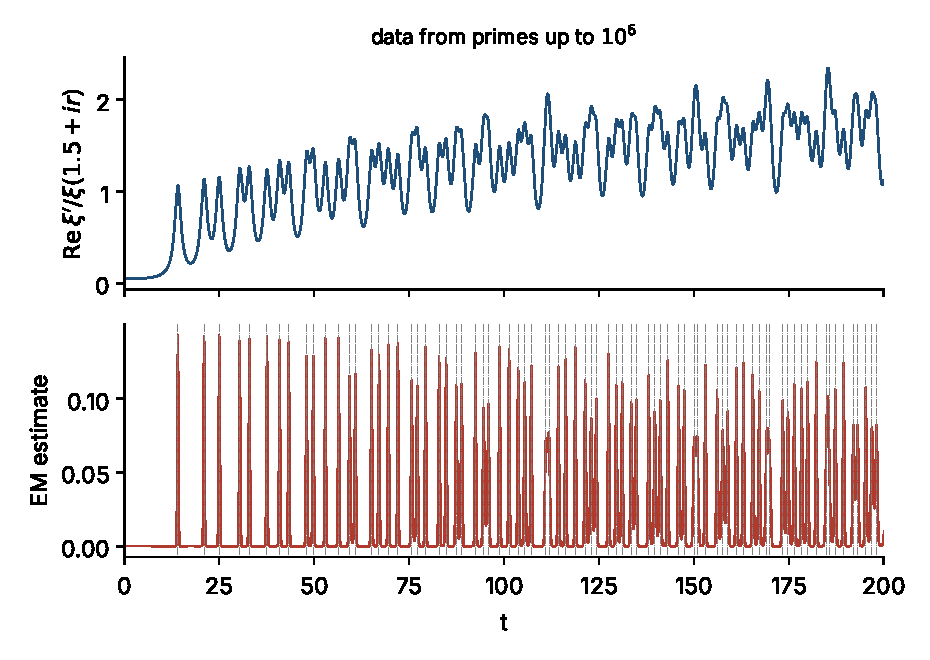
\includegraphics[width=\textwidth]{fig/v3/fig_p3_deconv.pdf}
% UNVERIFIED
\caption{Top: $\Re\,\xi'/\xi(1.5+ir)$ computed from the primes up to $10^6$. Bottom: the nonnegative EM deconvolution, with the ordinates of the zeros dotted.}
\label{ct:fig:p3}
\end{figure}

\section{The oscillation term, the Bondesson budget and the ladder}\label{ct:sec:budget}

This section reads the Thorin density of the compensated reciprocal Xi function as a Gamma budget minus an oscillation, and records what that gives for the ladder. Most of the statements restate Volume I in a new variable; we say which. We write $t_\alpha(z)=\big(v_\alpha(r)-b_\alpha\big)/(2\pi r)$, $r=\sqrt z$, for the signed function at every level $\alpha>0$. It is a Thorin density exactly when it is nonnegative (Theorem~\ref{thm:poisson}).

\subsection{The pole cancels}
Let $J(s)=s\int_1^\infty(\psi(x)-x)x^{-s-1}\dd x=-\frac{\zeta'}{\zeta}(s)-1-\frac1{s-1}$, the Mellin transform of Chebyshev's error. The integral converges for $\Re s>\Theta$ and the right side continues it. It is analytic at $s=1$, with $J(1)=-1-\gamma$. Put
\[
G_\alpha(r)=\tfrac12\Big(\Re\psi_\Gamma\big(1+\tfrac{\alpha+ir}2\big)-\psi_\Gamma\big(1+\tfrac\alpha2\big)\Big)\ge0,\qquad
\mathrm{Osc}_\alpha(r)=\Re J(\alpha+ir)-J(\alpha).
\]
By the digamma series, $G_\alpha$ is the Bondesson Gamma term of Section~\ref{ct:sec:levy}.

\begin{theorem}[budget form of the Thorin density]\label{ct:thm:budget}
For every $\alpha>0$ and every real $r$ at which $\xi(\alpha+ir)\ne0$,
\[
2\pi r\,t_\alpha(r^2)=v_\alpha(r)-b_\alpha=G_\alpha(r)-\mathrm{Osc}_\alpha(r).
\]
Hence $t_\alpha\ge0$ if and only if the oscillation of the Mellin transform of $\psi(x)-x$ along the line $\Re s=\alpha$ never exceeds the Gamma budget: $\Re J(\alpha+ir)-J(\alpha)\le G_\alpha(r)$ for all $r$.
\end{theorem}
\begin{proof}
$\frac{\xi'}{\xi}(s)=\frac12\psi_\Gamma(1+\frac s2)+\frac1{s-1}-\frac12\log\pi+\frac{\zeta'}{\zeta}(s)$ and $\frac{\zeta'}{\zeta}(s)=-1-\frac1{s-1}-J(s)$. The two pole terms cancel, so $\frac{\xi'}{\xi}(s)=\frac12\psi_\Gamma(1+\frac s2)-J(s)-1-\frac12\log\pi$. Take real parts at $s=\alpha+ir$ and subtract the value at $r=0$.
\end{proof}
The three term splitting of Section~\ref{ct:sec:levy} (primes, pole, Gamma) hides this. Above level one the pole is the only negative term, below level one it turns positive and the prime term turns signed. In the variable $J$ the pole disappears and two objects remain, one archimedean and explicit, one arithmetic and oscillating. The identity agrees to better than $10^{-16}$ at test points on both sides of level one (computed).

\begin{corollary}[one sided bound for the oscillation]\label{ct:cor:oscbound}
For every $\alpha\ge1$ and real $r$,
\[
\Re J(\alpha+ir)-J(\alpha)\ \le\ G_\alpha(r)\ \le\ \tfrac14\log\Big(1+\frac{r^2}{(2+\alpha)^2}\Big)+\frac{1}{2+\alpha} .
\]
\end{corollary}
\begin{proof}
The first inequality is $t_\alpha\ge0$ for $\alpha\ge1$, which is Proposition~\ref{bp:prop:valpha} (the minimum of $v_\alpha$ at the origin; Garunk\v{s}tis \cite{Garunkstis02}) combined with Theorem~\ref{ct:thm:budget}. For the second, $\Re\psi_\Gamma(1+x+iy)-\psi_\Gamma(1+x)=\sum_{k\ge1}f(k+x)\le f(1+x)+\int_1^\infty f(t+x)\dd t$ with $f(v)=y^2/(v(v^2+y^2))\le1/v$, at $x=\alpha/2$, $y=r/2$.
\end{proof}
At $\alpha=1$ this reads $\Re J(1+ir)\le-1-\gamma+G_1(r)$: an explicit bound on the edge of the strip, with no zero free region beyond $\Re s=1$. It is the minimum at the origin of Volume I with a digamma estimate added, and no more.

\subsection{Saturation on the critical line}
\begin{proposition}\label{ct:prop:saturation}
For every real $r$ that is not the ordinate of a zero, $\Re J(\frac12+ir)-J(\frac12)=G_{1/2}(r)$.
\end{proposition}
\begin{proof}
$\xi(\frac12+ir)$ is real, so $\frac{\xi'}{\xi}(\frac12+ir)$ is purely imaginary, and $\frac{\xi'}{\xi}(\frac12)=0$ by the functional equation. Apply Theorem~\ref{ct:thm:budget}.
\end{proof}
This is the classical $\Re\frac{\zeta'}{\zeta}(\frac12+it)=-\theta'(t)$ in the present language (checked to $10^{-19}$, computed). On the critical line the oscillation of Chebyshev's error spends the whole Gamma budget, for $\alpha\ge1$ it spends less than the budget for $r\ne0$, and RH says it never spends more for any $\alpha>\frac12$. Under RH, to first order in $\alpha-\frac12$ the condition is $\sum_\rho(r-\gamma)^{-2}\ge\sum_\rho\gamma^{-2}=q=0.0462100$ for all $r$, the sums over all zeros. This is the log concavity between zeros of the canonical product $\mathcal E$ of Conjecture~\ref{ct:conj:canonical}, and it holds whenever the gap containing $r$ is shorter than $\sqrt{8/q}=13.158$ (computed). It is the first order condition behind that conjecture.

How close is the race? Figure~\ref{ct:fig:budget} plots the share $\mathrm{Osc}_\alpha/G_\alpha$ of the budget used. At $r=1$ the share is $99.77\%$ at $\alpha=1$, $98.6\%$ at $\alpha=2$ and $99.97\%$ at $\alpha=0.6$ (computed). Positivity at small $r$ is decided by a fraction of a percent, because both sides vanish like $r^2$ and their difference is the contribution of the zeros, which are far away ($\gamma_1=14.13$). Near each ordinate the share swings far below zero, since there the zero adds a large positive peak to $t_\alpha$.

\begin{figure}[t]
\centering
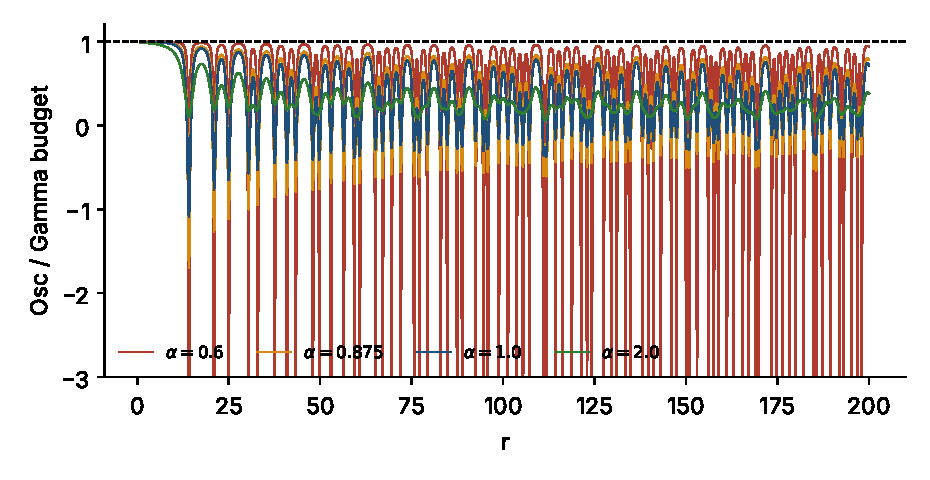
\includegraphics[width=\textwidth]{fig/v3/fig_budget.pdf}
\caption{Share of the Bondesson Gamma budget used by the Chebyshev oscillation, $\mathrm{Osc}_\alpha(r)/G_\alpha(r)$, at four levels. Positivity of the Thorin density is the statement that the curves stay below $1$.}
\label{ct:fig:budget}
\end{figure}

\subsection{The ladder and $\Theta$}
\begin{proposition}[the ladder is positive exactly down to $\Theta$]\label{ct:prop:qrh}
Let $\frac12\le\theta<1$. If no zero of $\zeta$ has real part greater than $\theta$, then $t_\alpha\ge0$ for every $\alpha>\theta$, so every rung above $\theta$ is the Laplace exponent of a GGC. Conversely, if $t_\alpha\ge0$ for every $\alpha>\theta$, then no zero has real part greater than $\theta$. Hence $\Theta=\inf\{\theta:\ t_\alpha\ge0\text{ for all }\alpha>\theta\}$.
\end{proposition}
This is not new. The direct part is Garunk\v{s}tis \cite{Garunkstis02} (for $\alpha\ge1$ it is Proposition~\ref{bp:prop:valpha}), and the converse is Theorem~\ref{thm:poisson} and Theorem~\ref{thm:dbeta:minall}(vi). The note of Polson proves the direct part again in three ranges of $r$: the convexity step of Proposition~\ref{bp:prop:v1min} for $r\le13.557$, a computed sum over the first $1545$ zeros on $[10,500]$ (double precision, not certified; the margin over the target $qa$ is $0.058a$, computed, attained at $r=10$), and above $500$ a counting argument in a window of half width $H=8.75$. An on line zero in the window pays at least $a/(\frac14+H^2)$, so $3.55$ zeros suffice, and an off line pair pays at least $a/(1+H^2)$, so $7.17$ counted zeros suffice (computed: $q(\frac14+H^2)=3.55$ and $2q(1+H^2)=7.17$). The explicit counting bound of Hasanalizade, Shen and Wong \cite{HSW22} supplies these counts (the note used Trudgian's bound, whose proof is incomplete; with it we recompute $4.77$ at $r=500$ and $61.58$ at $3\times10^{12}$). % UNVERIFIED: the counts from HSW22 at r=500 were not recomputed here.

Three consequences.
\begin{enumerate}
\item No further computation is needed once a zero free half plane is available. By the theorem of \cite{OAI26a} (Section~\ref{qrh:sec:claims}), $t_\alpha\ge0$ for every $\alpha>\frac78$ and the compensated reciprocal Xi function is a GGC on every such rung (proved). Below $\frac78$ the same implication is conditional on a zero free half plane of the corresponding width.
\item The supremum $\Theta$ of the real parts of the zeros, the error exponent of the prime number theorem ($\psi(x)-x=O(x^{\Theta+\epsilon})$), the abscissa of convergence of $J$ and the bottom of the positive Thorin ladder are one number.
\item In budget form: no zero has real part above $\theta$ if and only if the oscillation of $J$ stays within the Bondesson budget on every line to the right of $\theta$.
\end{enumerate}
Nothing here lowers $\Theta$. To lower $\theta$ one must bound $\mathrm{Osc}_\alpha$ on lines where the integral for $J$ is not known to converge, and every tool above runs the other way: a zero free half plane gives positivity, and positivity at level $\alpha$ says nothing at level $\alpha-\delta$, because a zero with real part between them is visible only through a term of size $\delta/((\alpha-\beta)^2+(r-\gamma)^2)$ that positivity does not bound. A genuine improvement would need an independent upper bound for $\Re J(\alpha+ir)$ inside the strip, uniform in $r$, of size $\frac12\log r$ (the growth of the budget). Convexity bounds for $\zeta'/\zeta$ are far weaker, which is the gap between zero density estimates and zero free regions.

\subsection{Far pairs and the origin}
Pairing each zero with its mirror image removes the restriction $\alpha\ge\frac12+10^{-8}$ that zeros above the verified height impose when they are bounded one at a time.
\begin{lemma}[far pairs pay]\label{ct:lem:farpair}
Let $\frac12<\alpha\le1$, let $\rho=\beta+i\gamma$ and $1-\bar\rho$ be zeros with $\gamma\ge100$ and $\beta>\frac12$, and put $a_1=\alpha-\beta$, $a_2=\alpha-1+\beta$, so that $a_1+a_2=2\alpha-1>0$ and $a_2>|a_1|$. For $0\le r\le\gamma/2$ the joint contribution of the two zeros and their conjugates to $v_\alpha(r)-v_\alpha(0)$ is nonnegative, whatever the sign of $a_1$.
\end{lemma}
\begin{proof}
With $P_a(d)=a/(a^2+d^2)$ the contribution of one zero and its conjugate is $F(a)=P_a(\gamma-r)+P_a(\gamma+r)-2P_a(\gamma)=a\,\varphi(a^2)$, where $\varphi(t)=\int_{-r}^r(r-|v|)f_t''(\gamma+v)\dd v$ and $f_t(x)=1/(t+x^2)$. For $x\ge50$ and $0\le t\le1$, $f_t''=(6x^2-2t)/(t+x^2)^3>0$ and $-\partial_tf_t''/f_t''\le4/x^2$, so $\varphi>0$ and $|\varphi'|\le(16/\gamma^2)\varphi$. Hence $H(a)=a\varphi(a^2)$ is odd and $H'(a)=\varphi+2a^2\varphi'\ge\varphi(1-32/\gamma^2)>0$ on $[0,1]$. Therefore $F(a_1)+F(a_2)=H(a_2)-H(|a_1|)\ge0$ when $a_1<0$, and both terms are nonnegative when $a_1\ge0$.
\end{proof}
In $1600$ random trials with $\gamma$ between $10^2$ and $3\times10^{12}$ the pair sum was never below $0.9995$ of its leading term $(2\alpha-1)\big((\gamma-r)^{-2}+(\gamma+r)^{-2}-2\gamma^{-2}\big)$ (computed; the smallest ratio was $0.99978$). The lemma gives positivity on every rung up to a finite height, but Theorem~\ref{thm:dbeta:minall}(ii) already states more (every $\alpha\in(\frac12,7.35]$ up to height $3\cdot10^{12}$), so we do not restate that.

\begin{proposition}[the origin is safe on every rung]\label{ct:prop:curv}
Unconditionally, for every $\frac12<\alpha<24$, $2\pi r\,t_\alpha(r^2)=\kappa(\alpha)r^2+O(r^4)$ as $r\to0$ with $\kappa(\alpha)=-\frac12\big(\frac{\xi'}{\xi}\big)''(\alpha)>0$, and the share of the budget used at the origin is $1-\kappa(\alpha)/g_2(\alpha)$ with $g_2(\alpha)=-\frac1{16}\psi_\Gamma''(1+\frac\alpha2)$.
\end{proposition}
\begin{proof}
Expand $v_\alpha(r)-b_\alpha=\kappa r^2+O(r^4)$. A zero with $a=\alpha-\beta$ contributes $a(3\gamma^2-a^2)/(a^2+\gamma^2)^3$ to $\kappa$. For $\alpha\le1$ the zeros up to the verified height are on the line, so $a\le\frac12$ and the contribution is positive, and the higher zeros contribute positively in pairs by the $r\to0$ form of Lemma~\ref{ct:lem:farpair}. For $1<\alpha<24$ every zero has $0<a<\alpha<\sqrt3\gamma_1=24.48$, so every term is positive. For larger $\alpha$ the term of $\gamma_1$ is negative and the argument stops.
\end{proof}
\begin{center}
\small
\begin{tabular}{lcccccc}
\toprule
$\alpha$ & $0.51$ & $0.6$ & $0.75$ & $0.875$ & $1.5$ & $2$\\
\midrule
$10^4\kappa(\alpha)$ & $0.0223$ & $0.223$ & $0.557$ & $0.835$ & $2.20$ & $3.25$\\
share at origin & $0.99997$ & $0.99970$ & $0.99914$ & $0.99855$ & $0.99373$ & $0.98713$\\
\bottomrule
\end{tabular}
\end{center}
(Computed.) To three digits $\kappa(\alpha)=2.23\times10^{-4}(\alpha-\frac12)$ near the line, which is $3(\alpha-\frac12)\sum_\rho\gamma^{-4}$ with the sum over all zeros: the slack that keeps $t_\alpha$ positive at the origin is a fourth moment of the zeros.

\section{The terms in factorial form}\label{ct:sec:factorial}

This section writes $\Re\frac{\xi'}{\xi}$ on the strip with the staircase $U$ of a Chebyshev combination kept bare, and says which Gamma function each term carries. The Mellin transform of the log factorial combination, the strip formula and the budget form are in Theorem~\ref{ct:thm:strip}, Proposition~\ref{ct:prop:mellincheb} and Theorem~\ref{ct:thm:budget}. What is added is the bare form, the Gamma bookkeeping and a comparison with Theorem~\ref{kr:thm:missing}. It follows an unrefereed note of Polson (November 2026).

Write $Z_U(s)=\zeta(s)P(s)=s\int_1^\infty U(x)x^{-s-1}\dd x$ for $\Re s>0$ (Theorem~\ref{ct:thm:strip}(1)), $R(x)=\prod_k\Gamma(1+c_kx)^{\varepsilon_k}$, and recall $P(1)=0$, $P'(1)=A$. By Stirling, $\log\lfloor y\rfloor!=\log\Gamma(1+y)-\{y\}\log y+O(1/y)$, so
\[
\begin{gathered}\sum_k\varepsilon_k\log\lfloor c_kx\rfloor!=\log R(x)+U(x)\log x+O(1),\\ \log R(x)=Ax+\tfrac12\Big(\sum_k\varepsilon_k\Big)\log x+O(1).\end{gathered}
\]
Differentiating $Z_U(s)/s$ in $s$ gives $s\int_1^\infty U(x)\log x\,x^{-s-1}\dd x=-Z_U'(s)+Z_U(s)/s$. Since $-\zeta'P=-Z_U'+\zeta P'$, the fractional parts $U\log x$ transform to $-Z_U'$ and the Stirling ratio $R$ transforms to $\zeta P'$, up to $Z_U/s$ and a bounded function, both analytic on $\Re s>0$. The pole of $\zeta P'$ at $s=1$ has residue $A$: Chebyshev's constant is the residue of the Stirling part (proved).

\begin{proposition}[factorial form]\label{ct:prop:factform}
For $s=\alpha+ir$ with $\alpha>0$, $s\ne1$ and $\zeta(s)P(s)\ne0$, in the chart of this chapter,
\[
2\pi r\,t^\circ_\alpha(r^2)=\Re\Big[\tfrac12\psi_\Gamma\big(1+\tfrac s2\big)+\frac1{s-1}-\tfrac12\log\pi+\frac{Z_U'}{Z_U}(s)-\frac{P'}{P}(s)\Big].
\]
\end{proposition}
\begin{proof}
$\frac{\zeta'}{\zeta}=\frac{(\zeta P)'}{\zeta P}-\frac{P'}{P}=\frac{Z_U'}{Z_U}-\frac{P'}{P}$. Insert this in the formula for $\xi'/\xi$ of Theorem~\ref{ct:thm:budget}.
\end{proof}
Here $t^\circ_\alpha$ is the signed function of Section~\ref{ct:sec:direct}. It is a Thorin density only when it is nonnegative, which for $\alpha>\Theta$ is automatic and below $\Theta$ presupposes the positivity being studied. The identity is meromorphic, so $P(s)=0$ is allowed whenever $\zeta(s)\ne0$ (at $s=1$ and for $P_R$ at $s=1+2\pi ik/\log2$ the two terms need a limit). It was confirmed to $10^{-50}$ at six points with $\Re s$ between $0.3$ and $2$ for both combinations, with $Z_U$ computed from the Hurwitz zeta function (computed). The three groups have three origins.
\begin{itemize}
\item $\frac12\psi_\Gamma(1+\frac s2)+\frac1{s-1}-\frac12\log\pi$ is archimedean. It comes from completing $\zeta$ to $\xi$ and owes nothing to the factorials. Its first term is the uncompensated form of the Bondesson term $G_\alpha$ of Section~\ref{ct:sec:budget}.
\item $Z_U'/Z_U$ is arithmetic. It is built from the staircase alone, by two integrals convergent on $\Re s>0$, and it is the only place the zeros of $\zeta$ enter.
\item $P'/P$ is elementary, a ratio of Dirichlet polynomials. It is all that remains of the Stirling Gamma function of the factorials.
\end{itemize}
For Ramanujan's combination $Z_U=\eta$ and $P_R(s)=1-2^{1-s}$ has zeros at $s=1+2\pi ik/\log2$, spacing $9.06$. They are zeros of $Z_U$ too, so at $\alpha=0.75$ the arithmetic and elementary terms have large spikes there of opposite sign, and the total is smooth (computed: at $r=9.0625$ the two terms are $-4.523$ and $+4.356$, the total is $0.021$). Away from $r=0$ and between zeros of $\zeta$ the arithmetic term is negative and the archimedean term pays for it; near $r=0$ it is positive up to about $r=2.6$ at $\alpha=0.75$ (computed).

With the convention of Theorem~\ref{ct:thm:budget} the compensated function subtracts the value at $r=0$: $2\pi r\,t_\alpha=2\pi r\,t^\circ_\alpha-b_\alpha=G_\alpha-\mathrm{Osc}_\alpha$. The proposition above is for $t^\circ_\alpha$, with no subtraction, and in the factorial form
\[
\mathrm{Osc}_\alpha(r)=-\Big[\Re\frac{Z_U'}{Z_U}-\Re\frac{P'}{P}+\Re\frac1{s-1}\Big]_{s=\alpha}^{s=\alpha+ir}.
\]
Positivity at a level $\alpha>\frac12$ is still the budget inequality of Theorem~\ref{ct:thm:budget}. It is proved for $\alpha\ge1$ and, by Theorem~\ref{thm:dbeta:minall}, for $\alpha>\frac12$ in the range there up to height $3\times10^{12}-1.21$; for all $\alpha>\frac12$ and all heights it is RH (Proposition~\ref{ct:prop:qrh}). Nothing here proves positivity below level one.

\begin{remark}[through the L\'evy density]\label{ct:rem:factlevy}
Put $\kappa(s)=\Gamma(s)Z_U(s)$, the cumulant function of Theorem~\ref{ct:thm:strip}(2), and $\mathbb E_s[\log y]=\kappa'(s)/\kappa(s)$ for real $s$ (for complex $s$ it is a ratio of oscillatory integrals). Legendre's duplication formula gives $\kappa(s)=2^s\pi^{(s-1)/2}\Gamma(\frac{s+1}2)\xi(s)P(s)/(s(s-1))$, hence
\[
\frac{\xi'}{\xi}(s)=\mathbb E_s[\log y]-\tfrac12\psi_\Gamma\big(\tfrac{s+1}2\big)-\frac{P'}{P}(s)+\frac1s+\frac1{s-1}-\log(2\sqrt\pi),
\]
and $\mathbb E_s[\log y]=\psi_\Gamma(s)+Z_U'/Z_U(s)$ (proved; confirmed to $10^{-16}$ or better, with limits set by quadrature at small $\Re s$ (computed)). This is a weaker variant of Theorem~\ref{kr:thm:missing}. The L\'evy density of Chebyshev's variable carries a full $\Gamma(s)$ while $\xi$ uses only $\Gamma(\frac s2)$, so the surplus $\Gamma(\frac{s+1}2)$ has to be divided out, whereas the Kolmogorov law of Theorem~\ref{kr:thm:missing} has the Gamma factor of $\xi$ and needs no such term. The last term $-P'/P$ is the term $-\log2/(2^{s-1}-1)$ there for $P_R$. The surplus is one of the two Gamma factors of the Mellin multiplier $\frac\pi{2\cos(\pi s/2)}=\frac12\Gamma(\frac{1+s}2)\Gamma(\frac{1-s}2)$ of the $2\sin^2$ transform (Theorem~\ref{ct:thm:strip}(3)).
\end{remark}
The Gamma content in $s$ of the four objects is: none for the log factorial combination in $x$ (it carries $-\zeta'P$); $\Gamma(\frac s2)\Gamma(\frac{s+1}2)$ for the L\'evy density; $\Gamma(\frac{1+s}2)\Gamma(\frac{1-s}2)$ for the Thorin deficit $\hat g$; and $\Gamma(\frac s2)$ for $\xi$. The L\'evy density and the Thorin deficit differ only in the Gamma factor; both carry $Z_U$.

\section{The direct form}\label{ct:sec:direct}

The compensated reciprocal $\xi(\alpha)e^{wb_\alpha}/\xi(\alpha+w)$ needed convexity, computation and counting. Without the compensator the positivity is a one line consequence of the Hadamard product, and this is Theorem~\ref{thm:poisson} and Proposition~\ref{bp:prop:valpha} of Volume I, which hold on the sharper range $\alpha>\Theta$ and with a converse. Only the mechanism for one pair of zeros is worth keeping here.

\begin{lemma}[one pair of zeros]\label{ct:lem:onepair}
Let $c=a-i\gamma$ with $a>0$. For $w\ge0$, $u=w^2$,
\[
\log\Big(1+\frac wc\Big)+\log\Big(1+\frac w{\bar c}\Big)=\int_0^\infty\log\Big(1+\frac uz\Big)\frac{P_a(r-\gamma)+P_a(r+\gamma)}{2\pi r}\dd z,\qquad r=\sqrt z,
\]
with $P_a(x)=a/(a^2+x^2)$. Hence $u\mapsto\dfrac{a^2+\gamma^2}{(a+\sqrt u)^2+\gamma^2}$ is the Laplace transform of a GGC with a strictly positive Thorin density.
\end{lemma}
\begin{proof}
$g(\zeta)=\log(1+w/\zeta)$ is analytic in $\Re\zeta>0$ with $\Re g(it)=\frac12\log(1+w^2/t^2)$, so the Poisson formula for the half plane gives $\Re g(a-i\gamma)=\frac1\pi\int_{-\infty}^\infty\frac12\log(1+w^2/t^2)P_a(t+\gamma)\dd t$. Fold the integral onto $t>0$ and put $z=t^2$.
\end{proof}
The identity holds to sixteen digits at $a=0.3$, $\gamma=14$, $w=1.7$ (computed; we found agreement to $10^{-32}$). In the variable $w$ the same factor is the transform of the signed density $\frac{a^2+\gamma^2}{\gamma}e^{-ax}\sin(\gamma x)$, which is not a probability law. Subordination by the stable law of index $\frac12$, which is what $w=\sqrt u$ does, turns each oscillating pair into a GGC. This is the $2\sin^2$ mechanism at the level of a single zero.

Summing over the conjugate pairs of the Hadamard product gives, for every $\alpha>\Theta$, the uncompensated density $t^\circ_\alpha(z)=\frac1{2\pi r}\,v_\alpha(r)>0$ with
\[
\frac{\xi(\alpha)}{\xi(\alpha+\sqrt u)}=\exp\Big(-\int_0^\infty\log\Big(1+\frac uz\Big)t^\circ_\alpha(z)\dd z\Big),
\]
as in Theorem~\ref{thm:poisson}. Two facts from Volume I and the note.
\begin{enumerate}
\item $t^\circ_\alpha=t_\alpha+\dfrac{b_\alpha}{2\pi r}$, and $b_\alpha/(2\pi r)$ is the Thorin density of the stable law of index $\frac12$ with Laplace transform $e^{-b_\alpha\sqrt u}$. So whenever $t_\alpha\ge0$ the uncompensated law is the independent sum of the compensated law and a stable component (Proposition~\ref{bp:prop:valpha}). Since $2\pi r\,t_\alpha\to0$ as $r\to0$, $b_\alpha$ is the largest stable component that can be split off, and $t_\alpha\ge0$ says that $\min_r v_\alpha(r)$ is attained at $r=0$.
\item Under RH at the centre every pair has $a=0$ and its factor is $(1+u/\gamma^2)^{-1}$, an exponential law of rate $\gamma^2$.
\end{enumerate}
Numerically $\log\xi(3)/\xi(2)=0.0917990$ and $\log\xi(4.5)/\xi(1.5)=0.342022$ (computed). The Thorin integral reproduces them only when the tail beyond $r=150$ is included: truncated at $r=150$ it gives $0.08737$ and $0.30215$, truncated at $3000$ it gives $0.091419$ and $0.338599$, and with the Riemann and von Mangoldt average density $\frac12\log(r/2\pi)$ beyond $3000$ it gives the exact values.

Inside the strip the direct proof fails at one point. A zero with $\beta>\alpha$ gives a pair with $a<0$, the Poisson kernel changes sign, and that pair is the reciprocal of a GGC factor. Showing directly that there is no such pair is RH. The primes cannot help in this form: the prime part of $t^\circ_\alpha$, namely $-\frac1{2\pi r}\sum_n\Lambda(n)n^{-\alpha}\cos(r\log n)$, is signed already for $\alpha>1$, so positivity is visible only on the zero side.

\section{Yamazato and Chebyshev in detail}\label{ct:sec:yamcheb}

\subsection{Yamazato's split carried out on the proved rung}
At $\alpha=1$ the function $F_1(r^2)=\frac1\pi(\arg\xi(1+ir)-b_1r)$ is nondecreasing (Proposition~\ref{bp:prop:v1min}), so the split is rigorous. We computed $F_1$ on $(0,600]$ with step $0.01$ (Figure~\ref{ct:fig:split}). All numbers are computed.
\begin{itemize}
\item The exponential series has $336$ rates with $r<600$, against $341$ zeros. The compensator removes $b_1r/\pi$ atoms, one for every $136$ units of height.
\item The mean of $X_1$ is $\frac12\big(\frac{\xi'}{\xi}\big)'(1)=0.023077$. On $[0,600]$ the exponential series carries $0.017615$ and the mixture of exponentials $0.003998$, so the mixture holds $18.5\%$ of the part of the mean carried on $[0,600]$. The rest of the mean, about $0.0015$, lies beyond $r=600$ and closes the sum.
\item The factorisation $\frac{\xi(1)}{\xi(1+w)}e^{b_1w}=\prod_n(1+u/\kappa_n)^{-1}\cdot\mathbb Ee^{-uY_1}$ is reproduced to six digits at $u=1,10,100$. At $u=100$ ($w=10$), $\log\frac{\xi(1+w)}{\xi(1)}-b_1w=2.131817$ directly, and the Thorin integral up to $600$ plus the Riemann and von Mangoldt tail gives $2.131824$. The values at $u=1,10$ are $0.023022$ and $0.227848$.
\end{itemize}
A correction to Section~\ref{ct:sec:yamazato} is needed at this level. That the half integer crossings of $F_\alpha$ are the zeros holds near the critical line and at low height. At $\alpha=1$ the drift $b_1r/\pi$ moves them steadily: the half integer crossings of $F_1$ differ from the zeros by $1.6$ units of $r$ at height $100$, $3.3$ at height $400$ and $5.2$ at height $590$. For the uncompensated function $F^\circ_\alpha=\frac1\pi\arg\xi(\alpha+ir)$ of Section~\ref{ct:sec:direct} there is no drift: at $\alpha=1$ it has $340$ atoms below $600$ and its half integer crossings stay within $0.51$ of all $341$ zeros.

\begin{figure}[t]
\centering
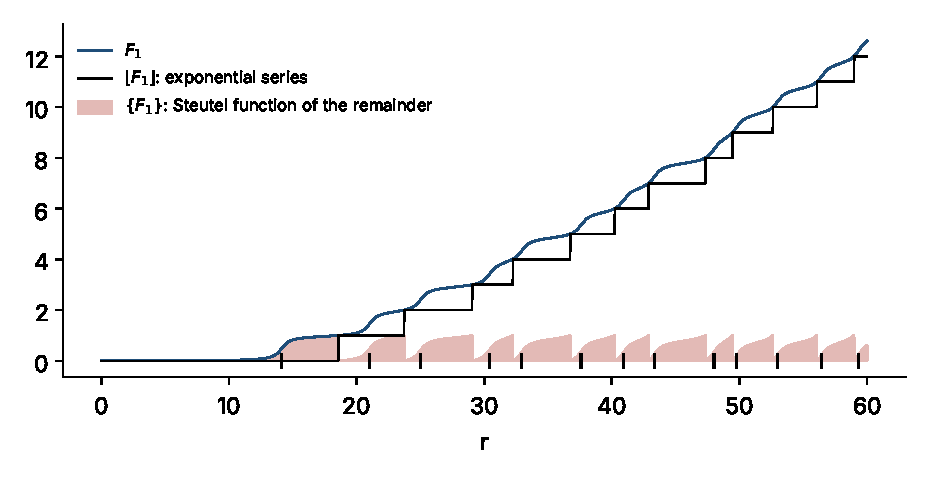
\includegraphics[width=\textwidth]{fig/v3/fig_yamazato_split.pdf}
\caption{Yamazato's split at level one. The staircase $\lfloor F_1\rfloor$ gives the exponential series; the shaded fractional part is the Steutel function of the mixture of exponentials. Ticks mark the zeros.}
\label{ct:fig:split}
\end{figure}

\subsection{The limit of the split at the critical line}
Under RH, as $\alpha\downarrow\frac12$ the rates tend to the critical points $r^*_n$ of the canonical product, not to the zeros (Conjecture~\ref{ct:conj:canonical}), so the split does not tend to the trivial one. Its limit is explicit under one more hypothesis, which the heuristic of the conjecture also uses: (H) each gap $(\gamma_n,\gamma_{n+1})$ contains exactly one critical point $r^*_n$ of $\mathcal E$. Hypothesis (H) holds for every gap shorter than $13.158$, hence for every gap up to the verified height.
\begin{proposition}[conditional on RH, simple zeros and (H)]\label{ct:prop:bernoulli}
As $\alpha\downarrow\frac12$ the Steutel function $\{F_\alpha\}$ tends pointwise to the indicator of $\bigcup_n(\gamma_n^2,r_n^{*2})$ in the variable $z$, and the split tends to
\[
\mathrm{Exp}\big(\gamma_n^2\big)\ \stackrel{d}{=}\ \mathrm{Exp}\big(r_n^{*2}\big)+B_n\,\mathrm{Exp}\big(\gamma_n^2\big),\qquad P(B_n=1)=1-\frac{\gamma_n^2}{r_n^{*2}},
\]
independently for each $n$: Yamazato's exponential series has the faster rates $r_n^{*2}$, and the remainder is a sum of Bernoulli thinned exponentials at the true rates.
\end{proposition}
\begin{proof}
At fixed $r$ between $\gamma_n$ and $\gamma_{n+1}$, $F_\alpha=n-\frac{\alpha-1/2}{\pi}\big(\frac{\Xi'}{\Xi}(r)+qr\big)+O((\alpha-\frac12)^2)$, and by (H) the bracket is positive before $r^*_n$ and negative after. So $\{F_\alpha\}\to1$ on $(\gamma_n,r^*_n)$ and $\to0$ on $(r^*_n,\gamma_{n+1})$. The passage to the laws is dominated convergence, since $0\le\{F_\alpha\}\le1$ (near $z=0$, under RH, $0\le F_\alpha(r^2)\le C(\alpha-\frac12)r^3$ for $r\le\gamma_1/2$, since every term of $v_\alpha(s)-b_\alpha$ is at most $(\alpha-\frac12)\,O(s^2\gamma^{-4})$, so the integrand $\min(1,Cz^{3/2})\,u/(z(z+u))$ dominates; this uses only the fixed $r$ expansion, not the uniformity in $r$ that Conjecture~\ref{ct:conj:canonical} leaves open). A Steutel function $\mathbf 1_{(\lambda,\mu)}$ has L\'evy density $(e^{-y\lambda}-e^{-y\mu})/y$, hence Laplace transform $\frac{1+u/\mu}{1+u/\lambda}=\frac\lambda\mu+\big(1-\frac\lambda\mu\big)\frac1{1+u/\lambda}$, with $\lambda=\gamma_n^2$, $\mu=r_n^{*2}$.
% TODO for the authors: confirm the wording of this domination bound (review M1)
\end{proof}
Without (H) the limit of $\{F_\alpha\}$ is the indicator of a different set and $r^*_n$ is undefined. The probabilities for the first eight zeros are $0.419,\allowbreak0.212,\allowbreak0.257,\allowbreak0.105,\allowbreak0.193,\allowbreak0.123,\allowbreak0.084,\allowbreak0.159$ (computed; $r_1^*=18.54500$ and $P(B_1=1)=0.41907$); over the first hundred they average $0.043$ and fall as low as $0.006$. Over those hundred zeros the exponential series carries $80.7\%$ of the mean and the Bernoulli remainder $19.3\%$. This is comparable with the $18.5\%$ at level one, but the two figures refer to different ranges and are not the same quantity. Yamazato's canonical form is thus close to stable along the ladder, but it is not the decomposition by zeros: it trades each zero for a slightly faster exponential plus a rare correction. The decomposition by zeros is the one in Section~\ref{ct:sec:direct}.

\subsection{Chebyshev's theorem in Mellin form}
Let $D(x)=\sum_{n\le x}u(n)\big(\psi(x/n)-x/n\big)$ be Chebyshev's weighted error (equation~\eqref{ct:eq:uweighted}) and $P(s)=1-2^{-s}-3^{-s}-5^{-s}+30^{-s}$.
\begin{proposition}\label{ct:prop:mellincheb}
$M_C(s):=s\int_1^\infty D(x)x^{-s-1}\dd x=\zeta(s)P(s)J(s)=-\zeta'(s)P(s)-\zeta(s)P(s)\frac{s}{s-1}$. It is analytic for $\Re s>0$, including at $s=1$ and at every zero of $\zeta$, and $J(s)=M_C(s)/(\zeta(s)P(s))$.
\end{proposition}
\begin{proof}
$s\int_1^\infty\mathbf 1\{x\ge N\}x^{-s-1}\dd x=N^{-s}$ and $s\int_1^\infty\mathbf 1\{x\ge n\}\frac xnx^{-s-1}\dd x=n^{-s}\frac s{s-1}$. The Dirichlet series of $\sum u(n)\psi(x/n)$ is $\zeta P\cdot(-\zeta'/\zeta)=-\zeta'P$, and $\sum u(n)n^{-s}=\zeta P$. Analyticity in $\Re s>0$ follows from $D(x)=(U(x)-\frac12)\log x+O(1)$, equation~\eqref{ct:eq:uweighted}.
\end{proof}
The zeros of $\zeta$ cancel in $-\zeta'P$, so no combination of factorials with finitely many divisors detects a zero. Numerically $|M_C(\rho_1)|=1.955$ at the first zero (computed). Chebyshev's weighted error is $O(\log x)$, which is why $M_C$ is analytic and of moderate size on every line in $\Re s>0$. That does not bound $J$: $J=M_C/(\zeta P)$ and $M_C=-\zeta'P-\zeta Ps/(s-1)$ needs $\zeta$ and $\zeta'$ on the line, so the difficulty has moved into the denominator, into the zeros of $\zeta$, and the zeros of $P$ cancel against those of $M_C$. Refining the weights, as Sylvester did, changes $P$ and $M_C$ together and leaves $J$ unchanged.

\subsection{Five objects in Yamazato form}
\begin{center}
\small
\begin{tabular}{p{0.27\textwidth}p{0.3\textwidth}p{0.33\textwidth}}
\toprule
object & Steutel function & split\\
\midrule
$\Gamma(1+w)e^{\gamma w}$ & $\lfloor z\rfloor$ & pure exponential series (Gumbel)\\
Chebyshev ratio $e^{-Aw}R(w)$ & $U(z)\in\{0,1\}$, periodic & pure mixture of exponentials\\
M\"obius limit $e^{-w}R_\mu(w)$ & $\mathbf 1\{z\ge1\}$ & one exponential, no remainder\\
$\xi(\frac12)/\xi(\frac12+w)$ under RH & $N(r)$ & pure exponential series at rates $\gamma^2$\\
rung $\alpha>\Theta$ & Gamma phase minus oscillation phase & rates at integer crossings plus mixture\\
\bottomrule
\end{tabular}
\end{center}
The first three live in the variable $w$ and the last two in $u=w^2$. Chebyshev's combination and the M\"obius limit are the two extremes of one family: in the first the Stirling parts cancel and only the periodic function $U$ is left, in the second $U$ has been replaced by a single indicator and a single atom remains. The truncated M\"obius combinations of Section~\ref{ct:sec:mobius} interpolate. On the Xi side the centre is pure atoms and at level one the remainder holds $18.5\%$ of the part of the mean carried on $[0,600]$ (computed).

\section{Chebyshev in the critical strip}\label{ct:sec:strip}

Chebyshev's identity is usually read at level one. This section shows that his floor combination reaches the whole critical strip, in three steps: the factorials, the Gamma function, and the $2\sin^2$ transform. The outcome is a formula for $\zeta$ on the strip as the Mellin transform of a Thorin deficit, and a positive even kernel for $\Xi$.

We use two combinations. Chebyshev's has $P_C(s)=1-2^{-s}-3^{-s}-5^{-s}+30^{-s}$ and $A_C=0.92129$. Ramanujan's has $d=(1,2)$, $\varepsilon=(1,-2)$, $U_R(t)=\lfloor t\rfloor-2\lfloor t/2\rfloor$, $A_R=\log2$ and
\[
P_R(s)=1-2^{1-s},\qquad\zeta(s)P_R(s)=\sum_{n\ge1}\frac{(-1)^{n-1}}{n^s}=\eta(s),
\]
so the combination Ramanujan used for Bertrand's postulate is Dirichlet's eta function. For a Chebyshev combination write $g(y)=\sum_nu(n)e^{-ny}$, $\hat g(r)=\int_0^\infty\cos(ry)g(y)\dd y=\sum_nu(n)\frac{n}{n^2+r^2}$, and recall from Theorem~\ref{ct:thm:chebggc} that $2\pi r\,t_C(r^2)=A-\hat g(r)$.

\begin{theorem}[three steps into the strip]\label{ct:thm:strip}
Let $U$ be the floor combination of a Chebyshev combination, bounded because $\sum\varepsilon_kc_k=0$.
\begin{enumerate}
\item Factorials. For $\Re s>0$, $\zeta(s)P(s)=s\int_1^\infty U(x)\,x^{-s-1}\dd x$. If $U\in\{0,1\}$ with up jumps at $n_j$ and down jumps at $m_j$, this is the alternating series $\sum_j(n_j^{-s}-m_j^{-s})$. For Chebyshev the jumps over one period are up at $1,7,11,13,17,19,23,29$ and down at $6,10,12,15,18,20,24,30$.
\item Yamazato and Gamma. The L\'evy density $\nu_C(y)=\int_0^\infty e^{-yz}U(z)\dd z$ of Theorem~\ref{ct:thm:chebME} satisfies, for $\Re s>0$,
\[
\int_0^\infty y^{s}\,\nu_C(y)\dd y=\Gamma(s)\,\zeta(s)\,P(s).
\]
At $s=m$ the left side is the $m$th cumulant of $X_C$, so $\Gamma(s)\zeta(s)P(s)$ is the cumulant function of Chebyshev's variable continued to fractional order.
\item The $2\sin^2$ transform. For $0<\Re s<1$,
\[
\int_0^\infty r^{-s}\,\hat g(r)\dd r=\frac{\pi}{2\cos(\pi s/2)}\,\zeta(s)\,P(s).
\]
\end{enumerate}
\end{theorem}
\begin{proof}
(1) Abel summation of $\sum u(n)n^{-s}=\zeta(s)P(s)$; the integral converges for $\Re s>0$ because $U$ is bounded. (2) $\int_0^\infty y^se^{-yz}\dd y=\Gamma(s+1)z^{-s-1}$, then (1). (3) $\hat g(r)=\sum_nu(n)\frac n{n^2+r^2}$ and $\int_0^\infty r^{-s}\frac{n}{n^2+r^2}\dd r=\frac{\pi}{2\cos(\pi s/2)}n^{-s}$ for $-1<\Re s<1$; sum over $n$ by Abel summation.
\end{proof}
All three identities were checked for both combinations at $s=\frac12$ and $s=\frac34+3i$ (computed): (1) to $10^{-25}$, (2) to $10^{-16}$ and (3) to $10^{-12}$.

So each step moves the same information, the staircase $U$, into a different object: a Dirichlet series, a L\'evy measure, a Thorin deficit. The Gamma function appears where Yamazato's remainder is turned into moments, and $\frac\pi{2\cos(\pi s/2)}=\frac12\Gamma(\frac{1+s}2)\Gamma(\frac{1-s}2)$ is the price of the $2\sin^2$ transform. Taking the logarithmic derivative of (3) gives $\zeta'/\zeta$ on the strip.
\begin{corollary}\label{ct:cor:stripdensity}
For $0<\Re s<1$ with $\zeta(s)P(s)\ne0$, put $\langle\log\rangle_s=\int_0^\infty r^{-s}\log r\,\hat g(r)\dd r\Big/\int_0^\infty r^{-s}\hat g(r)\dd r$. Then
\[
\frac{\zeta'}{\zeta}(s)=-\frac\pi2\tan\frac{\pi s}2-\langle\log\rangle_s-\frac{P'}{P}(s),
\]
and therefore, at every level $0<\alpha<1$, the signed function $t^\circ_\alpha$ of Section~\ref{ct:sec:direct} is
\[
t^\circ_\alpha(z)=\frac1{2\pi r}\,\Re\Big[\tfrac12\psi_\Gamma\big(1+\tfrac s2\big)+\frac1{s-1}-\tfrac12\log\pi-\frac\pi2\tan\frac{\pi s}2-\frac{P'}{P}(s)-\langle\log\rangle_s\Big]_{s=\alpha+ir}.
\]
\end{corollary}
The formula for $\zeta'/\zeta$ is confirmed to $10^{-10}$ at $s=\frac12$ and $s=\frac34+3i$ (computed). It is an identity for the signed function. By Theorem~\ref{thm:poisson}, $t^\circ_\alpha$ is a Thorin density only when no zero has real part above $\alpha$: for $\alpha<\frac12$ it is negative near $r=0$ unconditionally, and for $\frac12<\alpha<\Theta$ it is not a density at all. Every term except the last is elementary, and the last is a mean of $\log r$ under the complex weight $r^{-s}\hat g(r)$, the Thorin deficit of Chebyshev's or Ramanujan's ratio, tilted. Unlike the prime sum for $\Re\zeta'/\zeta$, which stops converging at level one, these integrals converge on the whole strip.

\subsection{Positivity: Ramanujan's combination is better than Chebyshev's}
\begin{proposition}\label{ct:prop:polya}
For Ramanujan's combination $g_R(y)=1/(e^y+1)$ is decreasing, convex and integrable, so its cosine transform $\hat g_R(r)=\log2-\Re\psi_\Gamma(1+ir)+\Re\psi_\Gamma(1+\frac{ir}2)$ is nonnegative. Hence on the strip
\[
\frac{\pi}{2\cos(\pi s/2)}\,(1-2^{1-s})\,\zeta(s)=\int_{-\infty}^\infty e^{(1-s)x}\,\hat g_R(e^x)\dd x
\]
is the two sided Laplace transform of a positive function, and on the critical line it is the Fourier transform of the positive kernel $K_R(x)=e^{x/2}\hat g_R(e^x)$. Since $P_R$ has no zeros in the open strip, RH is equivalent to: the Fourier transform of $K_R$ has no zeros with $0<|\Im t|<\frac12$.
\end{proposition}
The fact used is the classical positivity of the cosine transform of a convex decreasing integrable function (Young, P\'olya). For Chebyshev's combination the corresponding statement fails: $g_C$ is not monotone and $\hat g_C$ dips to $-0.0155$ at $r=7.55$ (computed), so the Thorin density of his ratio overshoots its tail constant $A$ slightly. In this respect the two term combination is the cleaner object, even though its Chebyshev constant $\log2=0.693$ is worse than $0.921$. For real $\sigma\in(0,1)$ the weight $r^{-\sigma}\hat g_R(r)$ is a probability density after normalisation, and Corollary~\ref{ct:cor:stripdensity} reads $-\frac{\zeta'}{\zeta}(\sigma)=\frac\pi2\tan\frac{\pi\sigma}2+\mathbb E_\sigma[\log r]+\frac{P_R'}{P_R}(\sigma)$.

What this does not give is a proof of positivity of $t^\circ_\alpha$ below level one. Three obstacles are specific. The tilt is complex: for real $s$ the mean $\langle\log\rangle_s$ is an expectation, but on the line $\alpha+ir$ it is a ratio of oscillatory integrals whose real part is not controlled by positivity of $\hat g$. The kernel $K_R$ decays only like $e^{x/2}$ on one side and $e^{-3x/2}$ on the other, so its Fourier transform decays like $e^{-\pi|t|/2}$ along the line, and the zeros cannot be seen numerically from $K_R$ at any useful height: at $t=17$ the transform has size $1.7\times10^{-11}$ (computed). Finally the standard real zero criteria (P\'olya, de Bruijn) need symmetry and faster decay, which Riemann's kernel $\Phi$ has and this one lacks. The next subsection supplies both.

\subsection{A symmetric kernel: the Gaussian step}
The Cauchy kernel of the $2\sin^2$ transform made $K_R$ lopsided and slowly decaying. Replace it by a Gaussian. Let
\begin{multline*}
\Theta_R(y)=\sum_{n\ge1}(-1)^{n-1}e^{-\pi n^2y}=\tfrac12\big(1-\vartheta_4(y)\big),\\
\int_0^\infty y^{s/2-1}\Theta_R(y)\dd y=\pi^{-s/2}\Gamma(\tfrac s2)\,\eta(s)\quad(\Re s>0),
\end{multline*}
which needs no subtraction at $y=0$, unlike Riemann's theta integral, because the weights have removed the pole. This Mellin identity is in Volume I (Section~\ref{sec:ch16:max}): $\vartheta_4(2k^2/\pi)=\Pr(K\le k)$ for the Kolmogorov law $K$, so $\Theta_R(y)=\frac12\Pr(K>\sqrt{\pi y/2})$, and $(1-2^{1-s})\zeta(s)=\mathbb E[(2K^2)^{s/2}]/(2\Gamma(1+\frac s2))$ is a case of the dictionary of Biane, Pitman and Yor \cite{BPY01}. The functional equation exchanges $P_R(s)=1-2^{1-s}$ with $P_R(1-s)=1-2^s$, so the symmetric object is $\Lambda(s)P_R(s)P_R(1-s)$ with $\Lambda(s)=\pi^{-s/2}\Gamma(\frac s2)\zeta(s)$, and multiplication by $P_R(1-s)$ is a dilation of the kernel. What is added to Volume I is this dilation, which makes the kernel even, and the explicit formula for $\Xi$.
\begin{theorem}[a positive even kernel for $\Xi$ from Ramanujan's combination]\label{ct:thm:symkernel}
Let $\Phi_R(x)=2e^{x/2}\big(\Theta_R(e^{2x}/4)-\Theta_R(e^{2x})\big)$. Then $\Phi_R$ is even and strictly positive, $\Phi_R(x)\sim2e^{|x|/2}\exp(-\frac\pi4e^{2|x|})$ as $|x|\to\infty$, and for every $t$
\[
\Xi(t)=\xi(\tfrac12+it)=\frac{t^2+\frac14}{2\,\big(3-2\sqrt2\cos(t\log2)\big)}\int_{-\infty}^\infty\Phi_R(x)\cos(tx)\dd x .
\]
\end{theorem}
\begin{proof}
$\int_0^\infty y^{s/2-1}\Theta_R(y/4)\dd y=2^s\Lambda(s)P_R(s)$, so $\Psi_R(y)=\Theta_R(y)-\Theta_R(y/4)$ has Mellin transform $\Lambda(s)P_R(s)(1-2^s)$, an entire function symmetric under $s\mapsto1-s$; hence $\Psi_R(1/y)=\sqrt y\,\Psi_R(y)$. Since $\vartheta_4(y)=\prod_n(1-q^{2n})(1-q^{2n-1})^2$ with $q=e^{-\pi y}$ increases in $y$, $\Theta_R$ decreases and $\Psi_R<0$, and $\Phi_R(x)=-2e^{x/2}\Psi_R(e^{2x})$. Put $y=e^{2x}$, $s=\frac12+it$, and use $\Lambda(\frac12+it)=-2\Xi(t)/(t^2+\frac14)$ and $|P_R(\frac12+it)|^2=3-2\sqrt2\cos(t\log2)>0$. The asymptotics come from the leading term $e^{-\pi y/4}$ of $\Theta_R(y/4)$.
\end{proof}
The self duality $\Phi_R(x)=\Phi_R(-x)$ holds to $10^{-42}$, the formula reproduces $\Xi(t)$ to thirty four digits at $t=0,5,20,40$ (for example $\Xi(20)=-3.665542775560946\times10^{-5}$ on both sides), and the thirteen sign changes of $F_R(t)=\int\Phi_R(x)\cos(tx)\dd x$ on $[0,60]$ are the first thirteen zeros of $\zeta$ to twelve decimals (all computed; Figure~\ref{ct:fig:symkernel}). So the instability of the Cauchy version is gone: with a Gaussian step the zeros are visible directly.

\begin{figure}[t]
\centering
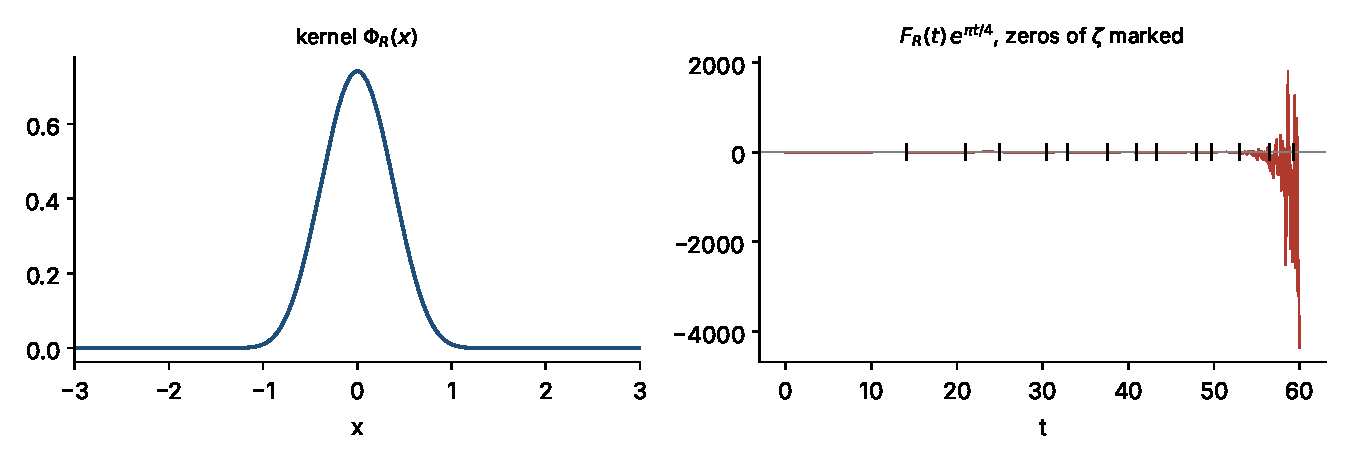
\includegraphics[width=\textwidth]{fig/v3/fig_symmetric_kernel.pdf}
\caption{Left: the kernel $\Phi_R$ built from Ramanujan's combination. Right: its cosine transform, rescaled, with the zeros of $\zeta$ marked.}
\label{ct:fig:symkernel}
\end{figure}

Compared with Riemann's kernel $\Phi(x)=2\sum_n(2\pi^2n^4e^{9x/2}-3\pi n^2e^{5x/2})e^{-\pi n^2e^{2x}}$ (equation~\eqref{eq:ch2:Phi} of Volume I, so that $\Xi(t)=\int\Phi(x)\cos(tx)\dd x$), this one involves no derivatives of the theta function: the pole is removed by Chebyshev type weights instead of by the factor $s(s-1)$. Numerically $\Phi_R$ is decreasing on $x>0$ and log concave, with $(\log\Phi_R)''\le-6.96$ on $(0,4)$, and $t\mapsto\log\Phi_R(\sqrt t)$ is concave as well, with second derivative at most $-0.86$ on $(0,8)$. Both are computed, not proved.

Two limits must be stated. First, RH is equivalent to $F_R$ having only real zeros in $|\Im t|<\frac12$, but $F_R$ also has zeros on $\Im t=\pm\frac12$, at $t=2\pi k/\log2\pm\frac i2$ with $k\ne0$, coming from $P_R(s)P_R(1-s)$. So $F_R$ is not in the Laguerre and P\'olya class whatever RH says, and the theory of de Bruijn and Newman cannot be applied to it as it stands: removing the pole arithmetically costs a row of zeros on the edge of the strip. Second, positivity, evenness and log concavity of a kernel do not by themselves force real zeros.

\section{Ramanujan's continuation and the $2\sin^2$ transform}\label{ct:sec:ramanujan}

Ramanujan's Master Theorem says that if $F(x)=\sum_{k\ge0}\varphi(k)(-x)^k/k!$ near the origin, then under growth conditions on $\varphi$ (Hardy) $\int_0^\infty x^{s-1}F(x)\dd x=\Gamma(s)\,\varphi(-s)$, and in the form without factorials, $F(x)=\sum_k\varphi(k)(-x)^k$ gives $\frac{\pi}{\sin\pi s}\varphi(-s)$. It is a continuation principle: the Taylor coefficients of $F$, a function on the integers, are interpolated to complex argument by the Mellin transform. The identities of Theorem~\ref{ct:thm:strip} are instances of it. We prove them directly, so the master theorem is used here as an interpretation and its growth conditions are not needed.

\begin{theorem}[the two Ramanujan continuations]\label{ct:thm:rmt}
For a Chebyshev combination with bounded $U$ and period $L=\mathrm{lcm}\{d\}$, with $g$ and $\hat g$ as in Section~\ref{ct:sec:strip},
\begin{align*}
g(y)&=\sum_{k\ge0}\zeta(-k)P(-k)\,\frac{(-y)^k}{k!},&\int_0^\infty y^{s-1}g\,\dd y&=\Gamma(s)\,\zeta(s)P(s),\\
\hat g(r)&=\sum_{k\ge0}\zeta(2k+1)P(2k+1)\,(-r^2)^k,&\int_0^\infty r^{-s}\hat g\,\dd r&=\frac{\pi\,\zeta(s)P(s)}{2\cos(\pi s/2)},
\end{align*}
the first series for $|y|<2\pi/L$ and the second for $|r|<1$, with the convention $\zeta(1)P(1)=A$.
\end{theorem}
\begin{proof}
The Mellin identities are Theorem~\ref{ct:thm:strip}. For the series, $\sum_nu(n)n^k$ is Abel summable to $\zeta(-k)P(-k)$, and $\frac n{n^2+r^2}=\sum_k(-1)^kr^{2k}n^{-2k-1}$. In the second case put $x=r^2$, $\varphi(k)=\zeta(2k+1)P(2k+1)$: the master theorem gives $\frac{\pi}{\sin\pi\sigma}\varphi(-\sigma)$ with $s=1-2\sigma$, which is $\frac{\pi}{\cos(\pi s/2)}\zeta(s)P(s)$, twice the integral in $r$.
\end{proof}
For Ramanujan's combination the first line is the classical $\frac1{e^y+1}=\sum_k\eta(-k)(-y)^k/k!$ and the second is $\hat g_R(r)=\log2-\eta(3)r^2+\eta(5)r^4-\cdots$ with $\eta(3)=0.90154$, $\eta(5)=0.97212$; the series for $\hat g_R$ agrees with the function to $25$ digits and the series for $1/(e^y+1)$ to $14$ digits at the test points (computed).

\subsection{What the $2\sin^2$ transform does}
\begin{enumerate}
\item It moves the interpolation nodes across the strip. On the L\'evy side the Taylor data are the values of $\zeta P$ at $0,-1,-2,\ldots$, to the left of the strip (Bernoulli numbers). On the Thorin side they are the values at the odd integers $1,3,5,\ldots$, to the right of it. The two continuations agree up to the explicit multiplier $\Gamma(1-s)\sin\frac{\pi s}2$, the Mellin transform of the cosine kernel and a factor of the functional equation of $\zeta$.
\item It turns the Thorin density into a generating function of odd zeta values: for $r=\sqrt z<1$,
\[
2\pi r\,t_C(z)=\sum_{k\ge1}(-1)^{k+1}\zeta(2k+1)P(2k+1)\,r^{2k}.
\]
For a single Gamma factor this is the classical expansion $\Re\psi_\Gamma(1+ir)+\gamma=\sum_{k\ge1}(-1)^{k+1}\zeta(2k+1)r^{2k}$ of the Bondesson density. The Thorin measure of a Gamma ratio carries three pieces of arithmetic: Taylor coefficients at the origin that are odd zeta values, the tail constant $A=\lim_{s\to1}\zeta(s)P(s)$, and a Mellin transform equal to $\zeta P$ on the critical strip.
\item It makes the strip a region of convergence. Neither series converges at $s$ in the strip and the prime sum does not either, but the Mellin integral of the Thorin deficit does, because $\hat g$ is bounded at the origin and $O(r^{-2})$ at infinity ($g$ is analytic at $0$ with $g(0)=\frac12$).
\end{enumerate}

\subsection{The same continuation on the Xi side}
At the centre, under RH, $\log\frac{\xi(\frac12+\sqrt u)}{\xi(\frac12)}=\sum_{\gamma>0}\log(1+u/\gamma^2)=\sum_{k\ge1}\frac{(-1)^{k+1}}{k}Z(k)u^k$, where $Z(s)=\sum_{\gamma>0}\gamma^{-2s}$ is the secondary zeta function of Voros \cite{Voros10}. The master theorem interpolates the coefficients.
\begin{proposition}\label{ct:prop:secondary}
Assume RH. For $\frac12<\Re s<1$,
\[
\int_0^\infty z^{-s}\,U_{1/2}(\dd z)=Z(s),\qquad
\int_0^\infty u^{-s-1}\log\frac{\xi(\frac12+\sqrt u)}{\xi(\frac12)}\dd u=\frac{\pi}{s\sin\pi s}\,Z(s),
\]
where $U_{1/2}=\sum_{\gamma>0}\delta_{\gamma^2}$.
\end{proposition}
\begin{proof}
$\int_0^\infty u^{-s-1}\log(1+u/z)\dd u=\frac{\pi}{s\sin\pi s}z^{-s}$ for $0<\Re s<1$; the sum over zeros converges for $\Re s>\frac12$.
\end{proof}
At $s=0.75$ the integral side is $1.46769$ (computed) and the formula side agrees to $10^{-4}$, the gap coming from the tail of the zero sum, which we estimated crudely. There is an exact parallel.
\begin{center}
\small
\begin{tabular}{p{0.2\textwidth}p{0.36\textwidth}p{0.34\textwidth}}
\toprule
& Gamma ratio (Chebyshev, Ramanujan) & reciprocal Xi at the centre\\
\midrule
Thorin object & deficit $\hat g(r)=A-2\pi rt_C$ & measure $U_{1/2}=\sum\delta_{\gamma^2}$\\
Taylor data & $\zeta(2k+1)P(2k+1)$ & $Z(k)=\sum\gamma^{-2k}$\\
Mellin transform & $\frac{\pi}{2\cos(\pi s/2)}\zeta(s)P(s)$ on $0<\Re s<1$ & $Z(s)$ on $\Re s>\frac12$\\
what it encodes & zeros of $\zeta$ as zeros of the transform & zeros of $\zeta$ as atoms of the measure\\
\bottomrule
\end{tabular}
\end{center}
On the left the zeros are where a Mellin transform vanishes, on the right they are where a measure sits. The Thorin programme of these volumes works on the right, and Chebyshev's and Ramanujan's Gamma ratios give the left side of the same picture.

\subsection{Implications and limits}
The $2\sin^2$ lemma is not only a positivity device: on the Mellin side it is multiplication by $\Gamma(1-s)\sin\frac{\pi s}2$, it carries Bernoulli number data to odd zeta value data, and it is the step at which the functional equation enters. For Thorin measures the Mellin transform is the natural invariant: for Gamma ratios it is $\zeta P$, for the reciprocal Xi at the centre it is the zeta function of the zeros, and for a rung $\alpha>\Theta$ it is $\int z^{-s}t^\circ_\alpha(z)\dd z$, which Corollary~\ref{ct:cor:stripdensity} makes computable from the first column. The limit is that the master theorem interpolates and does not locate zeros. Knowing $\zeta$ at the odd integers and continuing determines $\zeta$ in the strip, but in the ill conditioned way seen in Section~\ref{ct:sec:strip}, and nothing in the continuation constrains where the interpolated function vanishes. Is there a path to RH here? Not from the continuation itself. What it adds is a dictionary in which positivity of a Thorin measure, the functional equation and the values of $\zeta$ at integers are statements about one Mellin transform.

\section{Signed combinations: a strict hierarchy and linear programs}\label{ct:sec:hier}

This section and the next two are from a second unrefereed note of Polson (November 2026) on Chebyshev's factorial identity. They concern a general Chebyshev combination: weights $a_d$ on divisors $d$ with $\sum_da_d/d=0$, $R(w)=\prod_d\Gamma(1+w/d)^{a_d}$, $U(t)=\sum_da_d\lfloor t/d\rfloor$, $u(n)=U(n)-U(n-1)$, $V(k)=\sum_{j\le k}U(j)$, period $L=\mathrm{lcm}\{d\}$, $g(y)=\sum_nu(n)e^{-ny}$ and $\hat g(r)=\sum_nu(n)\frac{n}{n^2+r^2}$ as in Section~\ref{ct:sec:strip}, with tail constant $A=-\sum_da_d\log d/d$. The proof of Theorem~\ref{ct:thm:chebggc} does not use $a_d\in\mathbb Z$ or $U\in\{0,1\}$ except for the sign of $g$: for any real weights, $2\pi r\,t(r^2)=\int_0^\infty(1-\cos ry)g(y)\dd y=A-\hat g(r)$ is the density of the signed measure of $1/R(\sqrt u)$, which is a GGC exactly when $t\ge0$.

\begin{theorem}[a strict hierarchy]\label{ct:thm:hier}
Put $N(q)=\sum_{n\le L}u(n)q^n$.
\begin{enumerate}
\item $t\ge0$ if and only if $\hat g$ is largest at the origin: $\sum_nu(n)\frac n{n^2+r^2}\le A$ for every $r$. (This is the definition of $t$ rewritten, not a condition in terms of $U$.)
\item $g(y)=N(e^{-y})/(1-e^{-Ly})$, so $g\ge0$ if and only if the polynomial $N$ is nonnegative on $[0,1]$, a condition decidable exactly by Sturm sequences.
\item $U\ge0\Rightarrow V\ge0\Rightarrow g\ge0\Rightarrow t\ge0\Rightarrow A\ge0$, and no implication reverses. The first, second and fourth separations below are exact up to the stated precision of the fourth value, the third is computed on a grid.
\end{enumerate}
\end{theorem}
\begin{proof}
(1) $\int_0^\infty\cos(ry)e^{-ny}\dd y=n/(n^2+r^2)$. (2) Sum the geometric series in each residue class modulo $L$. (3) The first implication is trivial. If $V(k)\ge0$ for $1\le k\le L$ then $V(k+mL)=V(k)+mV(L)\ge0$ for all $k$, and $g=(1-q)^2\sum_nV(n)q^n\ge0$ with $q=e^{-y}$. Then $g\ge0\Rightarrow t\ge0$ by the formula before the theorem, and $t\ge0\Rightarrow A\ge0$ by letting $r\to\infty$. The examples below separate the classes.
\end{proof}
The chain $V\ge0\Rightarrow g\ge0\Rightarrow t\ge0$ proves Theorem~\ref{ct:thm:runningsums} in two lines and makes its convexity argument unnecessary.

\begin{center}
\small
\begin{tabular}{@{}l@{\ }l@{\ }p{0.4\linewidth}@{}}
\toprule
separates & combination $\{d:a_d\}$ & witness\\
\midrule
$V$ from $U$ & $\{1:1,\ 2:-3,\ 4:2\}$ & $U=(1,-1,0,0)$, $V=(1,0,0,0)\ge0$\\
$g$ from $V$ & $\{1:1,\ 2:-2,\ 4:-2,\ 6:3\}$ & $\min V=-1$, $N\ge0$ on $[0,1]$, $A=0.4904$\\
$t$ from $g$ & $\{1:1,\ 2:-3,\ 6:3\}$ & $g(0+)=-\frac12$, $t\ge0$ on a grid, $A=0.1438$\\
$A$ from $t$ & $\{1:1,\ 2:-5,\ 3:2,\ 4:4,\ 12:-2\}$ & $A=0.0283$; $2\pi rt=-0.0033$ near $r=4.86$\\
\bottomrule
\end{tabular}
\end{center}
For the second row $L=12$, the values of $U$ over one period are $(1,\allowbreak 0,\allowbreak 1,\allowbreak -2,\allowbreak -1,\allowbreak 1,\allowbreak 2,\allowbreak -1,\allowbreak 0,\allowbreak -1,\allowbreak 0,\allowbreak 0)$, and $N(q)=\allowbreak q(q-1)^2(q^4-q^2+1)\allowbreak(q^4+q^3+3q^2+q+1)$, whose factors are positive on $[0,1]$, so $g\ge0$ exactly. For the third row $g(0+)$ is minus half the sum of the weights, $-\frac12$, a value that is approached and not attained, and $2\pi rt$ has minimum $7.7\times10^{-7}$ on a logarithmic grid in $[10^{-3},10^{3}]$ (computed, not proved). For the fourth row the negative value is computed to five digits, and it is the example of smallest $L^1$ norm of the weights with coefficients in $\{-5,\ldots,5\}$ on the divisors of $12$ (exhaustive search, computed).

The second row answers Open problem~\ref{ct:op:signed}: nonnegative running sums are sufficient but not necessary. That combination has $A=2\log2-\frac12\log6>0$, a floor combination that takes the values $-2$ and $2$, and $V=-1$ at $k=5$, yet $g\ge0$ exactly, so $1/R(\sqrt u)$ is a GGC. The exact condition for $g\ge0$ is $N\ge0$ on $[0,1]$, and $t\ge0$ is the weaker condition of part~(1). A necessary and sufficient condition on $U$ alone is still unknown.

\subsection{Sylvester's problem as a linear program}
With real coefficients the identity, Stirling and the Abel summation argument of Proposition~\ref{ct:prop:cheb1850} go through unchanged, and the lower bound $\psi(x)\ge Ax+O(\log x)$ needs only $U\le1$. On the divisors of $N$, maximising $A$ subject to $\sum a_d/d=0$ and $U(m)\le1$ for $m\le N$ is a linear program with $N$ constraints. We solved it in floating point, and an independent recomputation with a second solver reproduces every entry; the entries are computed, not certified.
\begin{center}
\small
\begin{tabular}{rccc}
\toprule
$N$ & $U\le1$ & $0\le U\le1$ & $U\le1$ and $t\ge0$\\
\midrule
$30$ & $0.921292$ & $0.921292$ & $0.921292$\\
$210$ & $0.921292$ & $0.921292$ & $0.921292$\\
$2310$ & $0.921292$ & $0.921292$ & $0.921292$\\
$30030$ & $0.940637$ & $0.921292$ & $0.940637$\\
\bottomrule
\end{tabular}
\end{center}
In the last column $t\ge0$ is imposed on a grid of $3000$ values of $r$ in $[10^{-3},10^6]$, and the constraint is not binding. Two conclusions. First, among combinations with $0\le U\le1$ on the divisors of $30030$, Chebyshev's 1850 combination is optimal: no combination of these factorials does better while keeping his positivity (computed). It is not optimal among combinations with $t\ge0$, since the last column is larger. Second, going beyond $A$ requires signed floor combinations: the optimum at $N=30030$ has $U$ as low as $-5.48$ and about sixty nonzero real coefficients, and on the grid it still satisfies $t\ge0$, so it appears to be a GGC although it is no longer a mixture of exponentials. If its coefficients, which we do not print, satisfy $U(m)\le1$ in exact arithmetic, the elementary bound $\psi(x)\ge0.940637\,x+O(\log x)$ would follow without the prime number theorem. We mark it computed: a floating point vertex is not a proof, and an exact rational certificate has not been made. Whether linear programs over larger $N$ approach $1$ without the prime number theorem is open (Problem~\ref{ct:op:sylvester}); Diamond and Erd\H{o}s approach $1$ with it.

\section{The law of Chebyshev's variable}\label{ct:sec:lawx}

For a combination with $0\le U\le1$ the variable $X_C$ of Theorem~\ref{ct:thm:chebME} has mean $A$, and its cumulants follow from Theorem~\ref{ct:thm:strip}(2): $\kappa_m=\int_0^\infty y^m\nu_C(y)\dd y=\Gamma(m)\zeta(m)P(m)$ for $m\ge2$, that is $\kappa_m=(m-1)!\,\zeta(m)P(m)$. For Chebyshev's combination $P(2)=1-\frac14-\frac19-\frac1{25}+\frac1{900}=\frac35$, so the variance is exactly $\pi^2/10=0.98696$, and $\kappa_3=1.99541$, $\kappa_4=5.99751$ (computed, confirmed by differentiating $\log(e^{-Aw}R(w))$ at zero).

At the other end, Stirling gives $\mathbb Ee^{-wX_C}=(2\pi w)^{-1/2}(1+O(1/w))$ as $w\to\infty$, because $\frac12\sum_k\varepsilon_k\log(2\pi c_k)=-\frac12\log2\pi$ when $\sum\varepsilon_k\log c_k=0$, which holds for Chebyshev's combination. Karamata's Tauberian theorem for the distribution function then gives
\[
P(X_C\le x)\sim\frac{\sqrt{2x}}{\pi},\qquad x\to0 .
\]
Talbot inversion of the Laplace transform confirms it: the ratio $P(X_C\le x)\big/(\sqrt{2x}/\pi)$ is $1.0001,\ 1.0012,\ 1.0117$ at $x=10^{-4},10^{-3},10^{-2}$ (computed). The law has no atom at $0$, in agreement with Theorem~\ref{ct:thm:chebME}, and its distribution function rises like a square root.

\section{The M\"obius limit: where the zeros enter}\label{ct:sec:mobius}

Chebyshev's five weights are a crude version of something exact. This section takes the limit and shows that the identity never sees the zeros of $\zeta$; they enter only when the identity is inverted. Section~\ref{ct:sec:yamcheb} showed the same from the Dirichlet series side.

\begin{theorem}[the M\"obius combination]\label{ct:thm:mobius}
Take $a_d=\mu(d)$ for all $d\ge1$ and $R_\mu(w)=\prod_d\Gamma(1+w/d)^{\mu(d)}$. Then
\begin{enumerate}
\item $u=1*\mu=\delta_1$, so $U(t)=1$ for every $t\ge1$, $g(y)=e^{-y}$, and the identity reads $\sum_n\mu(n)\log\lfloor x/n\rfloor!=\psi(x)$.
\item $\displaystyle\prod_{d\ge1}\Big(\Gamma(1+w/d)\,e^{\gamma w/d}\Big)^{\mu(d)}=\frac{e^{w}}{1+w}$ for $w>-1$, the product converging absolutely.
\item The limiting law is the unit exponential: $e^{-w}R_\mu(w)=1/(1+w)$ is its Laplace transform, with drift $1$, and $1/R_\mu(\sqrt u)$ is the Laplace transform of a GGC with Thorin density $t(z)=\dfrac{r}{2\pi(1+r^2)}\ge0$, $r=\sqrt z$, so that $2\pi r\,t\to1$.
\end{enumerate}
\end{theorem}
\begin{proof}
(1) $\sum_{d\mid n}\mu(d)=[n=1]$, and M\"obius inversion of $\log\lfloor x\rfloor!=\sum_n\psi(x/n)$. (2) $\log\Gamma(1+x)+\gamma x=\sum_{k\ge2}\zeta(k)(-x)^k/k$ for $|x|<1$ and $\sum_d\mu(d)d^{-k}=1/\zeta(k)$, so the logarithm of the product is $\sum_{k\ge2}(-w)^k/k=w-\log(1+w)$ for $|w|<1$. Both sides are analytic for $w>-1$, and the series over $d$ converges absolutely because each term is $O(w^2/d^2)$. Equivalently, apply M\"obius inversion to Weierstrass's product. (3) The factors $e^{\gamma w/d}$ can be dropped because $\sum_d\mu(d)/d=0$. The L\'evy density is $g(y)/y=e^{-y}/y$, and $\int_0^\infty(1-\cos ry)e^{-y}\dd y=1-\frac1{1+r^2}=\frac{r^2}{1+r^2}$.
\end{proof}
Both $\sum\mu(d)/d=0$ and the drift $-\sum_d\mu(d)\log d/d=1$ are equivalent to the prime number theorem (Landau). Numerically, $\sum_{d\le10^6}\mu(d)\big(\log\Gamma(1+w/d)+\gamma w/d\big)$ differs from $w-\log(1+w)$ by $3.8\times10^{-11}$ at $w=0.5$, $6.1\times10^{-10}$ at $w=2$ and $1.5\times10^{-8}$ at $w=10$, and the error behaves like $w^2N^{-3/2}$ for $10\le N\le10^6$, which is what $\sum_{d>N}\mu(d)/d^2$ gives under RH (all computed).

Every Chebyshev combination is a finite Dirichlet polynomial approximation $P(s)$ to $1/\zeta(s)$, its Gamma ratio approximates the exponential law $e^w/(1+w)$, and its constant $A=P'(1)$ approximates $1$. The rate at which the window can close is governed by the zeros.

\begin{theorem}[RH as a rate of approximation]\label{ct:thm:mobrate}
Let $m(t)=\sum_{d\le t}\mu(d)/d$. For $N\ge1$ let the truncated M\"obius combination be $a_d=\mu(d)$ for $d<N$ and $a_N=\mu(N)-N\,m(N)$, so that $\sum a_d/d=0$. Its Chebyshev constant is
\[
A_N=\sum_{d\le N}\frac{\mu(d)}{d}\log\frac Nd=\int_1^N m(t)\frac{\dd t}{t},\qquad 1-A_N=\int_N^\infty m(t)\frac{\dd t}{t},
\]
and RH holds if and only if $1-A_N=O(N^{-1/2+\epsilon})$ for every $\epsilon>0$.
\end{theorem}
\begin{proof}
The formula for $A_N$ is $-\sum a_d\log d/d$ with the correction term, and $\log(N/d)=\int_d^N\dd t/t$. By the prime number theorem with the de la Vall\'ee Poussin error term, $m(t)=O(e^{-c\sqrt{\log t}})$, so $\int_1^\infty|m(t)|\dd t/t<\infty$, and $\int_1^\infty m(t)\dd t/t=\lim_{s\downarrow0}\frac1{s\zeta(1+s)}=1$ by Abel's theorem, which gives the expression for $1-A_N$. If RH holds then $M(x)=\sum_{n\le x}\mu(n)=O(x^{1/2+\epsilon})$ (Littlewood \cite{Littlewood12}; Titchmarsh \cite[Section 14.25]{Titchmarsh}), hence $m(t)=O(t^{-1/2+\epsilon})$ by partial summation, and the tail integral has the same order. Conversely, by Fubini (justified by the absolute convergence above), $\int_1^\infty(1-A_N)N^{-s-1}\dd N=\frac1s-\frac1{s^2\zeta(1+s)}$ for $\Re s>0$. The bound makes the left side analytic for $\Re s>-\frac12$, so $1/\zeta$ is analytic for $\Re s>\frac12$.
\end{proof}
This is a smoothed form of Littlewood's classical equivalence of RH with $M(x)=O(x^{1/2+\epsilon})$, equivalently $m(x)=O(x^{-1/2+\epsilon})$: since $1-A_N=\int_N^\infty m(t)\dd t/t$ is a logarithmic average of $m$, the criterion is the same statement in another dress, as hard as RH and not a step towards it. We make no claim of novelty. The computed values are $A_{30}=1.0030213$, $A_{10^3}=1.0004069$, $A_{10^5}=0.9999753$, $A_{10^7}=0.9999973$, and $|1-A_N|\sqrt N\le0.0218$ for $100\le N\le10^7$, with the maximum $0.02174$ at $N=324209$; the root mean square of $1-A_N$ over half decades has log log slope $-0.501$ (Figure~\ref{ct:fig:mobrate}). The normalised density $2\pi r\,t_N$ of the truncated combination at $N=30$ lies within $0.0031$ of $r^2/(1+r^2)$ for $0.01\le r\le1000$, the gap at large $r$ being $A_{30}-1$ (computed); it agrees to four decimals only for $r$ up to about $2$.

\begin{figure}[t]
\centering
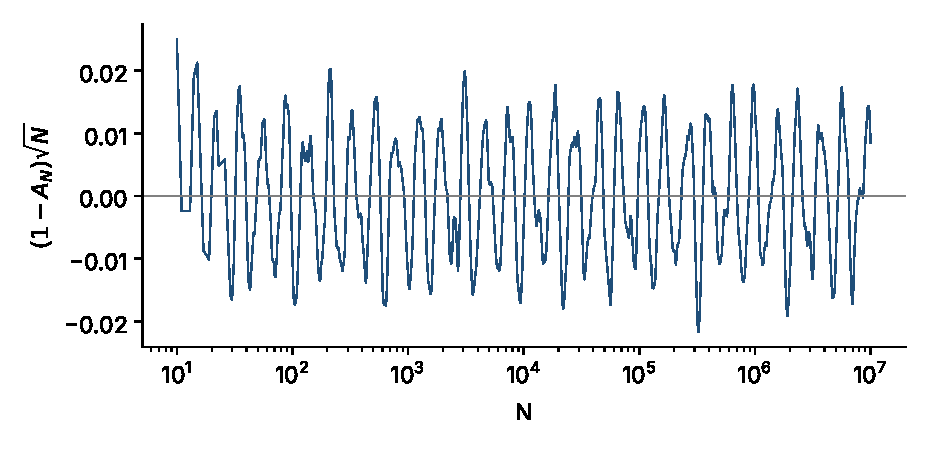
\includegraphics[width=\textwidth]{fig/v3/fig_mobius_rate.pdf}
\caption{$(1-A_N)\sqrt N$ for the truncated M\"obius combinations, $10\le N\le10^7$. Boundedness of this curve up to $N^{\epsilon}$ is equivalent to RH.}
\label{ct:fig:mobrate}
\end{figure}

\begin{remark}[what the limit does and does not give]
The truncated combination has $U_N=1$ on $[1,N)$, as good as possible, but beyond $N$ its floor combination leaves $[0,1]$: for $N=1000$ it ranges over $[-15.82,17.17]$ on $[N,20N]$ (computed). So $e^{-A_Nw}R_N(w)$ is not shown to be the Laplace transform of a law, and the running sum condition for the truncated stages has not been checked. We proved the limit object (Theorem~\ref{ct:thm:mobius}) and the rate criterion, but no theorem that the laws of Chebyshev combinations converge to the unit exponential. Chebyshev's Abel summation needs $U\le1$ everywhere, and that constraint holds his constant at $0.9213$ and the linear programming optimum at $0.9406$. A proof of anything about $\psi(x)-x$ along these lines would need a constrained approximation of $1/\zeta$ by Dirichlet polynomials whose error is controlled without knowing where the zeros are, and none is available.
\end{remark}

\section{What is proved, and the open problems}\label{ct:sec:path}

The chapter does not give a path to RH. Theorem~\ref{ct:thm:dictionary} turns RH into a statement about the primes, namely that the tapered transform $\int(1-\cos ru)e^{-\alpha u}M(\dd u)$ must converge for every $\alpha>\frac12$ (Theorem~\ref{thm:poisson}). The positivity of $t_\alpha$ for every $\alpha>\frac12$ is equivalent to RH, and on each line it implies the positivity of Lagarias. Every condition reached here is an equivalent of RH, not a step towards it. Precisely:
\begin{itemize}
\item Proved, in Volume I: $t_\alpha\ge0$ for every $\alpha\ge1$ (Propositions~\ref{bp:prop:v1min} and~\ref{bp:prop:valpha}); and unconditionally on $\frac12<\alpha\le7.35$ up to height $3\cdot10^{12}$ (Theorem~\ref{thm:dbeta:minall}(ii)).
\item Proved, conditional on RH: $t_\alpha\ge0$ for $\frac12<\alpha<1$ (Lagarias \cite{Lagarias}, Theorem~\ref{thm:dbeta:minall}).
\item The negative decomposition mass of the uncompensated density $v_\alpha/\pi$ for $\frac12<\alpha<1$ is bounded through the zero density estimate of Guth and Maynard \cite{GM26} in Theorem~\ref{ag:thm:almost}. A density bound gives no zero free half plane and so no positivity.
\item Heuristic: smoothing preserves positivity and deconvolution does not, so the descent from $\alpha=1$ is a Cauchy deconvolution of a line spectrum observed through a periodogram of Chebyshev's error, and the harmonic continuation of $v_\alpha$ towards the line is ill posed.
\item Proved here: Theorems~\ref{ct:thm:chebggc}, \ref{ct:thm:chebME} and~\ref{ct:thm:runningsums}, Corollary~\ref{ct:cor:bondesson}, Propositions~\ref{ct:prop:levy} and~\ref{ct:prop:yamxi}, with the numerical checks marked computed.
\item Certified here: the range II inequality of Section~\ref{ct:sec:rung}, margin $0.0900$.
\item Proved in the later sections: the budget identity (Theorem~\ref{ct:thm:budget}), the one sided oscillation bound for $\alpha\ge1$ (Corollary~\ref{ct:cor:oscbound}, a citation of Volume I with a digamma estimate), the strip identities (Theorem~\ref{ct:thm:strip}), the even kernel (Theorem~\ref{ct:thm:symkernel}) and the hierarchy of Theorem~\ref{ct:thm:hier} (the third separation is computed on a grid). Conditional on RH, simple zeros and (H): Proposition~\ref{ct:prop:bernoulli}. Known and restated: Proposition~\ref{ct:prop:qrh} (Garunk\v{s}tis and Theorem~\ref{thm:poisson}), Theorem~\ref{ct:thm:mobrate} (Littlewood's criterion in smoothed form).
\item Computed, floating point only: the linear program optimum $0.940637$ at $N=30030$ and the optimality of Chebyshev's combination among $0\le U\le1$ there.
\end{itemize}

\begin{problem}\label{ct:op:sylvester}
Over all weights $(\varepsilon_k,c_k)$ with $\sum\varepsilon_kc_k=0$ and nonnegative floor combination, maximise the lower Chebyshev constant subject to a bounded upper constant. Each feasible point is a GGC with explicit Thorin density; is the optimum a limit of GGCs whose Thorin measure converges to that of $\Gamma(s)\zeta(s)$ with the pole removed?
\end{problem}
\begin{problem}\label{ct:op:signed}
Characterise all finite signed products $\prod\Gamma(1+c_kw)^{\varepsilon_k}$ whose reciprocal at $\sqrt u$ is a GGC. Theorem~\ref{ct:thm:runningsums} is a sufficient condition. Whether nonnegativity of the running sums is also necessary is answered no by the combination $\{1:1,2:-2,4:-2,6:3\}$ of Theorem~\ref{ct:thm:hier}; a characterisation in terms of the floor combination alone remains open.
\end{problem}
\begin{problem}
Build a Bayesian line spectrum estimator for $U_{\rm RH}$ from $Z(u)$ on $[0,\log X]$ (Cauchy deconvolution with a positivity prior) and quantify the posterior resolution as a function of $X$. How large must $X$ be to certify the first $K$ atoms? The deconvolution of Section~\ref{ct:sec:deconv} gives no such statement.
\end{problem}
\begin{problem}
Make the extreme value heuristic rigorous for the rotor process: under LI, show that the record values of $Z$ on $[0,U]$ grow like $\frac{1}{2\pi}(\log\log U)^2$, and prove the saddlepoint step. Then transfer the statement from the rotor model to $Z(u)$.
\end{problem}
\begin{problem}
Prove Conjecture~\ref{ct:conj:canonical}: the uniformity in $r$ of the expansion in $\alpha-\frac12$, so that the Yamazato rates of the Thorin ladder converge to the critical points of the canonical product, and compare the rates at level one with them (the first ten differ from the critical points at $\alpha=\frac12$ by at most $0.16$ in $r$).
\end{problem}
